\documentclass[12pt,a4paper,oneside]{book}

% 1. Master Style for RBRU Zigbee AIoT Academic Manual (RBRU Masterclass Standard)
\usepackage{styles/zigbee_rbru_style}

% 2. Font configuration for XeLaTeX (Thai Unicode Sarabun)
\usepackage{fontspec}
\setmainfont{Sarabun}
\setsansfont{Sarabun}
\setmonofont{Sarabun}[Scale=0.9]

% 3. Hyperref Setup
\usepackage{hyperref}
\hypersetup{
    colorlinks=true,
    linkcolor=rbruNavy,
    citecolor=agriForest,
    urlcolor=meshCyan,
    filecolor=zigbeeAmber,
    pdftitle={คู่มือระบบสื่อสารไร้สาย Zigbee 3.0 สำหรับการเกษตรแม่นยำสูง - มหาวิทยาลัยราชภัฏรำไพพรรณี},
    pdfauthor={ผู้ช่วยศาสตราจารย์ ดร.ชีวะ ทัศนา}
}

\begin{document}

% ==========================================
% ส่วนนำ (Frontmatter)
% ==========================================
\frontmatter
% ============================================================
% ปกหน้าคู่มือวิชาการ (Academic Book Cover)
% มาตรฐาน มหาวิทยาลัยราชภัฏรำไพพรรณี (RBRU Masterclass)
% ============================================================
\thispagestyle{empty}
\begin{titlepage}
\begin{tikzpicture}[remember picture, overlay]
    % พื้นหลังหลักไล่ระดับสีน้ำเงินเข้มและสีเขียวป่าไม้
    \fill[left color=rbruNavy!98!black, right color=rbruNavy!88!agriForest] 
        (current page.south west) rectangle (current page.north east);
    
    % แถบขลิบทองราชภัฏแนวตั้งทางซ้าย
    \fill[color=rbruGold] 
        ([xshift=2.4cm]current page.south west) rectangle ([xshift=2.6cm]current page.north west);

    % เส้นเรขาคณิตเวกเตอร์คลื่นวิทยุโครงข่ายแบบโปร่งแสง
    \draw[color=white, opacity=0.08, line width=1.0pt]
        ([xshift=3.5cm, yshift=-2.5cm]current page.north west) -- ([xshift=-1.5cm, yshift=5cm]current page.south east);
    \draw[color=rbruGold, opacity=0.12, line width=1.2pt]
        ([xshift=3.5cm, yshift=-6cm]current page.north west) -- ([xshift=-1cm, yshift=2cm]current page.south east);

    % ข้อมูลสังกัดด้านบน
    \node[anchor=north west, text width=14.5cm] at ([xshift=3.2cm, yshift=-2.0cm]current page.north west) {
        {\fontsize{14}{18}\selectfont\bfseries\color{rbruGold} คณะวิทยาศาสตร์และเทคโนโลยี มหาวิทยาลัยราชภัฏรำไพพรรณี\par}
        \vspace{2pt}
        {\fontsize{10}{13}\selectfont\color{softMist!85} โครงการพัฒนาทักษะวิชาชีพชั้นสูงเพื่อการขับเคลื่อนเศรษฐกิจฐานนวัตกรรม (AIoT 2570)\par}
    };

    % ส่วนชื่อเรื่องหลัก (Main Title Block)
    \node[anchor=north west, text width=15.2cm] at ([xshift=3.2cm, yshift=-3.5cm]current page.north west) {
        {\color{rbruGold}\rule{0.45\textwidth}{3pt}\par}
        \vspace{8pt}
        {\fontsize{26}{33}\selectfont\bfseries\color{white} คู่มือระบบสื่อสารไร้สาย Zigbee 3.0\par}
        \vspace{3pt}
        {\fontsize{24}{31}\selectfont\bfseries\color{white} สำหรับการเกษตรแม่นยำสูง\par}
        \vspace{6pt}
        {\fontsize{14}{19}\selectfont\bfseries\color{zigbeeOrange} เครือข่ายแบบเมช เซนเซอร์เกษตร เกตเวย์ และไมโครคอนโทรลเลอร์ ESP32-C6\par}
        \vspace{4pt}
        {\fontsize{9}{13}\selectfont\color{softMist!85} Zigbee 3.0 Wireless Mesh Sensor Networks for Precision Agriculture Manual\\Mesh Topology, Industrial Sensors, MQTT Gateway, and ESP32-C6 Firmware Development\par}
        \vspace{8pt}
        {\color{rbruGold}\rule{0.75\textwidth}{1.2pt}\par}
    };

    % กรอบภาพศิลป์ปก Masterclass (Cover Artwork Window)
    \node[anchor=center, draw=rbruGold, line width=2.0pt, rounded corners=6pt, inner sep=0pt, fill=black] 
        at ([xshift=1.0cm, yshift=-1.1cm]current page.center) {
        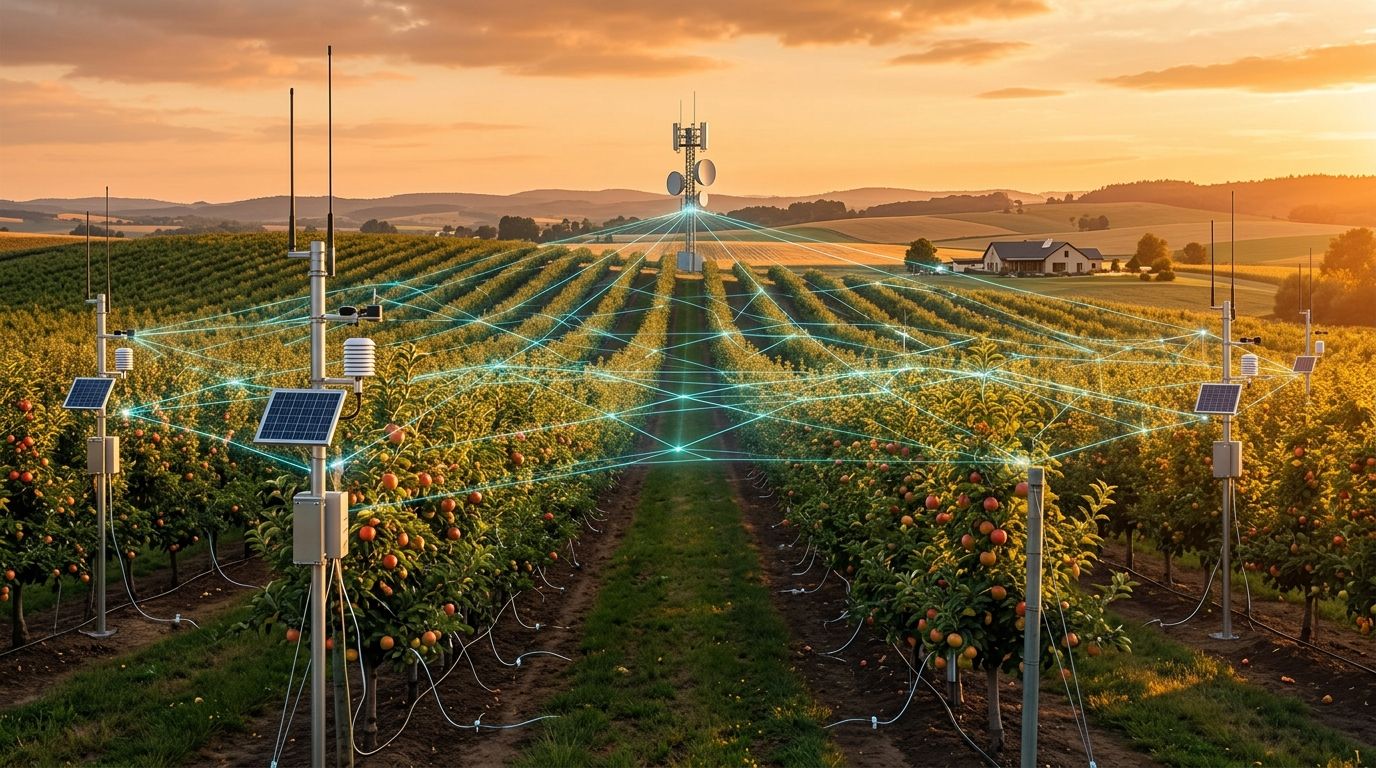
\includegraphics[width=14.5cm, height=9.0cm, keepaspectratio=false]{figures/zigbee_farm_mesh_realistic.jpg}
    };

    % รายนามคณะผู้เขียนและสำนักพิมพ์ด้านล่าง
    \node[anchor=south west, text width=14.5cm] at ([xshift=3.2cm, yshift=1.8cm]current page.south west) {
        {\fontsize{12}{15}\selectfont\bfseries\color{white} ผู้ช่วยศาสตราจารย์ ดร.ชีวะ ทัศนา\par}
        \vspace{2pt}
        {\fontsize{9.5}{12}\selectfont\color{softMist!90} กลุ่มวิจัยฟิสิกส์เกษตรดิจิทัลและปัญญาประดิษฐ์ฝังตัว\par}
        \vspace{2pt}
        {\fontsize{8.5}{11}\selectfont\color{softMist!75} คณะวิทยาศาสตร์และเทคโนโลยี มหาวิทยาลัยราชภัฏรำไพพรรณี\par}
        \vspace{10pt}
        {\color{rbruGold}\rule{0.35\textwidth}{0.8pt}\par}
        \vspace{4pt}
        {\fontsize{10}{13}\selectfont\bfseries\color{rbruGold} สำนักพิมพ์มหาวิทยาลัยราชภัฏรำไพพรรณี \quad \textbar \quad \color{softMist!80}พ.ศ. 2570\par}
    };
\end{tikzpicture}
\end{titlepage}
\clearpage

% ============================================================
% หน้าชื่อเรื่อง (Title Page)
% ============================================================
\thispagestyle{empty}
\begin{center}
    \vspace*{1.5cm}
    
    {\fontsize{24}{30}\selectfont\bfseries\color{rbruNavy} คู่มือระบบสื่อสารไร้สาย Zigbee 3.0\\สำหรับการเกษตรแม่นยำสูง\par}
    
    \vspace{0.8cm}
    {\fontsize{14}{20}\selectfont\bfseries\color{agriForest} สถาปัตยกรรมโครงข่ายแบบเมช ระบบนิเวศเซนเซอร์เกษตร\\เกตเวย์ Zigbee2MQTT และการพัฒนาเฟิร์มแวร์ ESP32-C6\par}
    
    \vspace{1.2cm}
    {\color{rbruGold}\rule{0.6\textwidth}{1.5pt}\par}
    
    \vspace{1.5cm}
    {\fontsize{16}{22}\selectfont\bfseries\color{charcoal} ผู้ช่วยศาสตราจารย์ ดร.ชีวะ ทัศนา\par}
    \vspace{0.3cm}
    {\fontsize{12}{16}\selectfont\color{slateGrey} วศ.ด. (วิศวกรรมไฟฟ้าและอิเล็กทรอนิกส์), วศ.ม. (วิศวกรรมโทรคมนาคม)\par}
    {\fontsize{12}{16}\selectfont\color{slateGrey} กลุ่มวิจัยฟิสิกส์เกษตรดิจิทัลและปัญญาประดิษฐ์ฝังตัว\par}
    
    \vfill
    
    {\fontsize{13}{18}\selectfont\bfseries\color{rbruNavy} คณะวิทยาศาสตร์และเทคโนโลยี มหาวิทยาลัยราชภัฏรำไพพรรณี\par}
    \vspace{0.2cm}
    {\fontsize{11}{15}\selectfont\color{slateGrey} เอกสารคู่มือวิชาการประกอบการฝึกอบรมเชิงปฏิบัติการขั้นสูง\\โครงการพัฒนาทักษะวิชาชีพชั้นสูงเพื่อการขับเคลื่อนเศรษฐกิจฐานนวัตกรรม (AIoT 2570)\par}
    \vspace{0.4cm}
    {\fontsize{11}{15}\selectfont\bfseries\color{rbruGold} พ.ศ. 2570\par}
\end{center}
\clearpage

% ============================================================
% คำนำ (Preface)
% ============================================================
\chapter*{คำนำ}
\addcontentsline{toc}{chapter}{คำนำ}

ระบบสื่อสารไร้สายในแปลงเกษตรกรรมสมัยใหม่ถือเป็นโครงสร้างพื้นฐานที่มีบทบาทสำคัญอย่างยิ่งต่อความแม่นยำในการเก็บรวบรวมข้อมูลโทรมาตรและการสั่งการอุปกรณ์ควบคุมอัตโนมัติ สภาพแวดล้อมทางการเกษตรในภูมิภาคเขตร้อนชื้น เช่น สวนผลไม้เศรษฐกิจและโรงเรือนปลูกพืช มักเผชิญกับอุปสรรคทางกายภาพจากการลดทอนของคลื่นวิทยุโดยทรงพุ่มใบพืชที่มีปริมาณน้ำสูง ตลอดจนระยะทางระหว่างโหนดตรวจวัดที่กระจายตัวในพื้นที่กว้าง เทคโนโลยีโครงข่ายแบบเมชตามมาตรฐาน Zigbee 3.0 บนพื้นฐานข้อกำหนด IEEE 802.15.4 จึงเป็นคำตอบทางวิศวกรรมที่เหมาะสมที่สุด ด้วยคุณสมบัติเด่นด้านการจัดเส้นทางเครือข่ายด้วยตนเอง การซ่อมแซมเส้นทางส่งสัญญาณแบบพลวัต และการประหยัดพลังงานอย่างสูงสุด

คู่มือวิชาการฉบับนี้เรียบเรียงขึ้นเพื่อเป็นเอกสารหลักในการศึกษา วิจัย และลงมือปฏิบัติการพัฒนาระบบสื่อสารไร้สาย Zigbee 3.0 สำหรับงานวิศวกรรมฟิสิกส์เกษตรแม่นยำ โดยมุ่งเน้นการถ่ายทอดองค์ความรู้ตั้งแต่ระดับรากฐานทางฟิสิกส์คลื่นวิทยุ การวิเคราะห์เปรียบเทียบเชิงสมรรถนะร่วมกับเทคโนโลยีอื่น การประยุกต์ใช้งานโหนดเซนเซอร์ตรวจวัดสภาพดิน สภาพบรรยากาศ และรังสีดวงอาทิตย์ การเชื่อมต่อกับหัววัดมาตรฐานอุตสาหกรรมผ่านสะพานสื่อสาร RS485 Modbus RTU ไปจนถึงการติดตั้งและบริหารจัดการเกตเวย์โครงข่ายร่วมกับ Zigbee2MQTT เพื่อบูรณาการข้อมูลสู่แพลตฟอร์มคลาวด์และระบบควบคุมฟาร์มอัจฉริยะ ตลอดจนการพัฒนาเฟิร์มแวร์บนไมโครคอนโทรลเลอร์รุ่นใหม่ ESP32-C6 สถาปัตยกรรม RISC-V

ผู้เรียบเรียงหวังเป็นอย่างยิ่งว่า คู่มือเล่มนี้จะเป็นประโยชน์ต่อนักศึกษา นักวิจัย วิศวกร ตลอดจนผู้สนใจในเทคโนโลยีอินเทอร์เน็ตของสรรพสิ่งทางการเกษตร เพื่อนำไปประยุกต์ใช้ในการยกระดับผลิตภาพทางการเกษตรและขับเคลื่อนนวัตกรรมเทคโนโลยีเกษตรกรรมดิจิทัลของประเทศให้ก้าวหน้าอย่างมั่นคงและยั่งยืน

\vspace{1.5cm}
\begin{flushright}
    \textbf{ผู้ช่วยศาสตราจารย์ ดร.ชีวะ ทัศนา}\\
    กลุ่มวิจัยฟิสิกส์เกษตรดิจิทัลและปัญญาประดิษฐ์ฝังตัว\\
    คณะวิทยาศาสตร์และเทคโนโลยี มหาวิทยาลัยราชภัฏรำไพพรรณี\\
    กันยายน 2570
\end{flushright}
\clearpage

% ============================================================
% แผนการสอนและประมวลรายวิชา (Course Syllabus)
% ============================================================
\chapter*{ประมวลรายวิชาและแผนการจัดการเรียนรู้}
\addcontentsline{toc}{chapter}{ประมวลรายวิชาและแผนการจัดการเรียนรู้}

\noindent\textbf{รหัสและชื่อวิชา} \quad AIOT4302 ระบบสื่อสารไร้สายและอินเทอร์เน็ตของสรรพสิ่งทางการเกษตร\\
(Wireless Communications and Agricultural Internet of Things)

\noindent\textbf{จำนวนหน่วยกิต} \quad 3(2-2-5) บรรยาย 2 ชั่วโมง ปฏิบัติการ 2 ชั่วโมง ศึกษาค้นคว้าด้วยตนเอง 5 ชั่วโมงต่อสัปดาห์

\noindent\textbf{คำอธิบายรายวิชา} \quad หลักการและสถาปัตยกรรมระบบสื่อสารไร้สายระยะสั้นและระยะปานกลางสำหรับงานเกษตรกรรมแม่นยำสูง โพรโทคอลเครือข่ายแบบเมชตามมาตรฐาน IEEE 802.15.4 และ Zigbee 3.0 สถาปัตยกรรมการจัดเส้นทางแบบพลวัต ระบบนิเวศเซนเซอร์ตรวจวัดดิน บรรยากาศ และรังสีแสง การเชื่อมโยงเซนเซอร์อุตสาหกรรมผ่านสะพานสื่อสาร RS485 Modbus RTU สถาปัตยกรรมเกตเวย์โครงข่ายร่วมกับ Zigbee2MQTT และโพรโทคอล MQTT การพัฒนาเฟิร์มแวร์ไมโครคอนโทรลเลอร์ ESP32-C6 สถาปัตยกรรม RISC-V การคำนวณและบริหารจัดการพลังงานต่ำ และการออกแบบโครงงานบูรณาการในแปลงเกษตรอัจฉริยะ

\vspace{0.4cm}
\noindent\textbf{แผนการจัดการเรียนรู้รายสัปดาห์}

\begin{table}[H]
\caption{แผนการจัดการเรียนรู้รายสัปดาห์ตลอดภาคการศึกษา}
\label{tab:syllabus_schedule}
\centering
\small
\begin{tabularx}{\textwidth}{c p{3.2cm} >{\raggedright\arraybackslash}X c}
\toprule
\textbf{สัปดาห์} & \textbf{หัวข้อเนื้อหา} & \textbf{กิจกรรมและการทดลองปฏิบัติการ} & \textbf{สื่อและอุปกรณ์} \\
\midrule
1 & รากฐานฟิสิกส์คลื่นวิทยุ & วิเคราะห์การลดทอนสัญญาณคลื่น 2.4 GHz ในแปลงเกษตร & เครื่องวิเคราะห์สเปกตรัม \\
2--3 & สถาปัตยกรรม Zigbee 3.0 & การกำหนดบทบาท Coordinator, Router และ End Device & ซอฟต์แวร์ Wireshark \\
4 & อัลกอริทึม AODV Routing & จำลองการจัดเส้นทางแบบเมชและการกู้คืนเครือข่าย & บอร์ดทดลอง CC2652P \\
5 & เปรียบเทียบมาตรฐานไร้สาย & ทดสอบสมรรถนะ Zigbee เทียบกับ LoRaWAN และ Wi-Fi & ชุดรับส่งสัญญาณทดสอบ \\
6--7 & เซนเซอร์ดินอัจฉริยะ & ติดตั้งโพรบวัดความชื้น อุณหภูมิ EC, pH และธาตุอาหาร NPK & โพรบดิน RS485 Modbus \\
8 & เซนเซอร์บรรยากาศและรังสี & บูรณาการหัววัด SHT30, BMP280 และโฟโตเซนเซอร์ PAR & สถานีสภาพอากาศจำลอง \\
9 & สะพานเชื่อมต่อ RS485 & พัฒนาเฟิร์มแวร์แปลงค่า Modbus RTU สู่โพรโทคอล Zigbee & โมดูล MAX485 และ MCU \\
10 & สอบวัดผลกลางภาค & ประเมินผลภาคทฤษฎีและทดสอบทักษะโครงข่ายเชิงปฏิบัติการ & ชุดข้อสอบและใบงาน \\
11 & เกตเวย์ Zigbee2MQTT & ติดตั้งและตั้งค่า Coordinator CC2652P บน Raspberry Pi & เกตเวย์คอมพิวเตอร์ \\
12 & โครงสร้างข้อมูล MQTT & กำหนดสเปกหัวข้อ JSON Telemetry และคำสั่งควบคุม Actuator & ซอฟต์แวร์ MQTT Explorer \\
13 & สถาปัตยกรรม ESP32-C6 & พัฒนาเฟิร์มแวร์ด้วย ESP-IDF และ ESPHome บนคลื่น 802.15.4 & บอร์ด ESP32-C6 DevKit \\
14 & การจัดการพลังงานต่ำ & ทดลอง Deep Sleep คำนวณแบตเตอรี่ และออกแบบโซลาร์เซลล์ & เครื่องวัดกระแสละเอียด \\
15 & โครงงานบูรณาการ & นำเสนอผลงานแปลงทดลองเสมือนจริง 120 โหนด และประเมินผล & แปลงทดสอบภาคสนาม \\
\bottomrule
\end{tabularx}
\end{table}

\clearpage


% สารบัญหลัก สารบัญภาพ และสารบัญตาราง
\clearpage
\phantomsection
\addcontentsline{toc}{chapter}{\contentsname}
\tableofcontents

\clearpage
\phantomsection
\addcontentsline{toc}{chapter}{\listfigurename}
\listoffigures

\clearpage
\phantomsection
\addcontentsline{toc}{chapter}{\listtablename}
\listoftables

% ==========================================
% ส่วนเนื้อหา (Mainmatter)
% ==========================================
\mainmatter

% บทที่ 1: สถาปัตยกรรมและโพรโทคอลเครือข่าย Zigbee 3.0
% ============================================================
% บทที่ 1: สถาปัตยกรรมและโพรโทคอลเครือข่าย Zigbee 3.0 สำหรับการเกษตรแม่นยำ
% ============================================================
\chapter[สถาปัตยกรรมและโพรโทคอลเครือข่าย Zigbee 3.0 สำหรับการเกษตรแม่นยำ]{สถาปัตยกรรมและโพรโทคอลเครือข่าย Zigbee 3.0\\สำหรับการเกษตรแม่นยำ}
\label{chap:ch01}

% ------------------------------------------------------------
% แผนบริหารการสอนประจำบทที่ 1 (หน้า 1/2)
% ------------------------------------------------------------
\section*{แผนบริหารการสอนประจำบทที่ 1}
\addcontentsline{toc}{section}{แผนบริหารการสอนประจำบทที่ 1}

\begin{planbox}{หัวข้อเนื้อหาประจำบท}
\begin{enumerate}[topsep=1pt, itemsep=0.5pt, partopsep=0pt, parsep=0pt, leftmargin=1.5em]
    \item รากฐานฟิสิกส์คลื่นวิทยุและการแพร่กระจายสัญญาณคลื่น 2.4 GHz ในทรงพุ่มแปลงเกษตร
    \item สถาปัตยกรรมและบทบาทของอุปกรณ์โครงข่ายตามมาตรฐาน Zigbee 3.0
    \item อัลกอริทึมการจัดเส้นทางแบบเมชและกลไกการซ่อมแซมโครงข่ายแบบพลวัต
    \item การวิเคราะห์เปรียบเทียบเชิงวิศวกรรมระหว่าง Zigbee 3.0, LoRaWAN, Wi-Fi และ BLE
    \item การออกแบบโครงสร้างโทโพโลยีแบบขยายขนาดได้สำหรับแปลงปลูกและโรงเรือนอัจฉริยะ
\end{enumerate}
\end{planbox}

\begin{planbox}{วัตถุประสงค์เชิงพฤติกรรม}
\begin{enumerate}[topsep=1pt, itemsep=0.5pt, partopsep=0pt, parsep=0pt, leftmargin=1.5em]
    \item อธิบายหลักการแพร่กระจายคลื่นและการสูญเสียกำลังส่งในแปลงเกษตรกรรมได้อย่างถูกต้อง
    \item จำแนกบทบาทและหน้าที่ของ Coordinator, Router และ End Device ได้อย่างแม่นยำ
    \item วิเคราะห์ขั้นตอนการค้นหาเส้นทางด้วยอัลกอริทึม AODV และการกู้คืนเครือข่ายได้
    \item เปรียบเทียบข้อได้เปรียบเชิงเทคนิคของระบบไร้สายแต่ละชนิดในงานฟาร์มอัจฉริยะได้
    \item ออกแบบแผนผังโครงข่ายแบบเมชรองรับพื้นที่แปลงเกษตรกรรมจริงได้อย่างมีประสิทธิภาพ
\end{enumerate}
\end{planbox}

\newpage

% ------------------------------------------------------------
% แผนบริหารการสอนประจำบทที่ 1 (หน้า 2/2)
% ------------------------------------------------------------
\begin{planbox}{วิธีสอนและกิจกรรมการเรียนการสอน}
\begin{enumerate}[topsep=1pt, itemsep=0.5pt, partopsep=0pt, parsep=0pt, leftmargin=1.5em]
    \item การบรรยายเชิงทฤษฎีควบคู่กับการยกตัวอย่างกรณีศึกษาแปลงเกษตรกรรมภาคตะวันออก
    \item การสาธิตการทำงานของโครงข่าย Zigbee Mesh ผ่านแบบจำลองและการดักจับแพ็กเก็ต
    \item การฝึกปฏิบัติการตรวจวัดความแรงสัญญาณ RSSI และ LQI ภายใต้สภาพแปลงปลูกจำลอง
    \item การจัดกิจกรรมกลุ่มเพื่อร่วมกันแก้โจทย์ปัญหาการเชื่อมต่อโหนดที่มีสิ่งกีดขวาง
    \item การมอบหมายงานศึกษาค้นคว้าอิสระและจัดทำรายงานวิเคราะห์โครงข่ายสื่อสาร
\end{enumerate}
\end{planbox}

\begin{planbox}{สื่อการเรียนการสอน}
\begin{enumerate}[topsep=1pt, itemsep=0.5pt, partopsep=0pt, parsep=0pt, leftmargin=1.5em]
    \item เอกสารประกอบการสอนวิชาสถาปัตยกรรมและโพรโทคอลเครือข่ายไร้สาย
    \item บอร์ดทดลองไมโครคอนโทรลเลอร์ CC2652P และ ESP32-C6 พร้อมเสาอากาศภายนอก
    \item ซอฟต์แวร์วิเคราะห์โครงข่าย Wireshark พร้อมอุปกรณ์ Zigbee Packet Sniffer
    \item วิดีทัศน์สาธิตการซ่อมแซมเส้นทางส่งสัญญาณเมื่อโหนดเราเตอร์หยุดทำงานกะทันหัน
    \item ผังโครงสร้างมาตรฐาน Zigbee Cluster Library และสเปกข้อกำหนดทางเทคนิค
\end{enumerate}
\end{planbox}

\begin{planbox}{การวัดและประเมินผล}
\begin{enumerate}[topsep=1pt, itemsep=0.5pt, partopsep=0pt, parsep=0pt, leftmargin=1.5em]
    \item การประเมินผลจากแบบทดสอบความรู้ก่อนเรียนและหลังเรียนประจำบท
    \item การประเมินทักษะการตั้งค่าอุปกรณ์และการดักจับแพ็กเก็ตในห้องปฏิบัติการ
    \item การประเมินคุณภาพรายงานการออกแบบโครงข่ายและการคำนวณงบประมาณการสูญเสียกำลัง
    \item การสังเกตพฤติกรรมการมีส่วนร่วมในการอภิปรายและการทำงานร่วมกันเป็นทีม
\end{enumerate}
\end{planbox}

\clearpage

% ------------------------------------------------------------
% เนื้อหาบทที่ 1
% ------------------------------------------------------------
\section{รากฐานฟิสิกส์คลื่นวิทยุและการลดทอนสัญญาณในแปลงเกษตรกรรม}

การส่งผ่านข้อมูลไร้สายในสภาพแวดล้อมทางการเกษตร \textbf{การแพร่กระจายคลื่นวิทยุ (Radio Frequency Propagation)}\index{Radio Propagation@Radio Propagation (การแพร่กระจายคลื่น)} ในย่านความถี่ ISM 2.4 GHz เผชิญกับความท้าทายทางกายภาพที่แตกต่างจากอาคารสำนักงานหรือพื้นที่โล่งทั่วไปอย่างสิ้นเชิง ทรงพุ่มใบพืช ลำต้น กิ่งก้าน ตลอดจนหยดน้ำค้างบนผิวใบ ล้วนมีพฤติกรรมเป็นตัวดูดกลืนและหักเหคลื่นแม่เหล็กไฟฟ้า ส่งผลให้คลื่นเกิดการลดทอนเชิงพื้นที่ (Path Loss)\index{Path Loss@Path Loss (การสูญเสียกำลังส่ง)} และการสะท้อนหลายเส้นทาง (Multipath Fading) อย่างมีนัยสำคัญ

การสูญเสียกำลังส่งในพื้นที่ว่าง (Free-Space Path Loss หรือ FSPL)\index{FSPL@FSPL (Free-Space Path Loss)} สำหรับคลื่นวิทยุที่มีความถี่ $f$ ในหน่วยเมกะเฮิร์ตซ์ และระยะทาง $d$ ในหน่วยกิโลเมตร สามารถคำนวณได้ตามแบบจำลองทางฟิสิกส์ดังสมการ
\begin{equation}
    \text{FSPL} = 20\log_{10}(d) + 20\log_{10}(f) + 32.44 \quad \text{[dB]}
\end{equation}

อย่างไรก็ดี ในแปลงปลูกพืชจริง ทรงพุ่มที่มีความหนาแน่นจะสร้างการลดทอนเพิ่มเติมตามแบบจำลอง \textbf{การลดทอนของฟิตซ์เจอรัลด์ (Modified Weissberger Model)} ซึ่งแสดงความสัมพันธ์ของการลดทอนจากใบพืช $L_{\text{veg}}$ ในหน่วยเดซิเบล สำหรับความลึกของทรงพุ่ม $d_f$ ในหน่วยเมตร ดังสมการ
\begin{equation}
    L_{\text{veg}} = 0.25 f^{0.39} d_f^{0.63} \quad \text{[dB]} \quad (14 < d_f \le 400)
\end{equation}
โดยที่ $f$ คือความถี่คลื่นในหน่วยกิกะเฮิร์ตซ์ ($f = 2.4$ GHz) จากสมการดังกล่าวจะเห็นได้ว่า เมื่อทรงพุ่มมีความหนาแน่นเพิ่มขึ้นในฤดูที่มีการผลิใบและติดผล สัญญาณคลื่นวิทยุจะลดทอนอย่างรวดเร็ว ส่งผลให้การเชื่อมต่อแบบจุดต่อจุดในระยะไกลไม่สามารถรักษาเสถียรภาพได้ การนำสถาปัตยกรรมโครงข่ายแบบเมชเข้ามาประยุกต์จึงเป็นทางเลือกเชิงวิศวกรรมที่มีประสิทธิภาพสูงสุด\index{Mesh Network@Mesh Network (โครงข่ายแบบเมช)}

\begin{figure}[H]
    \centering
    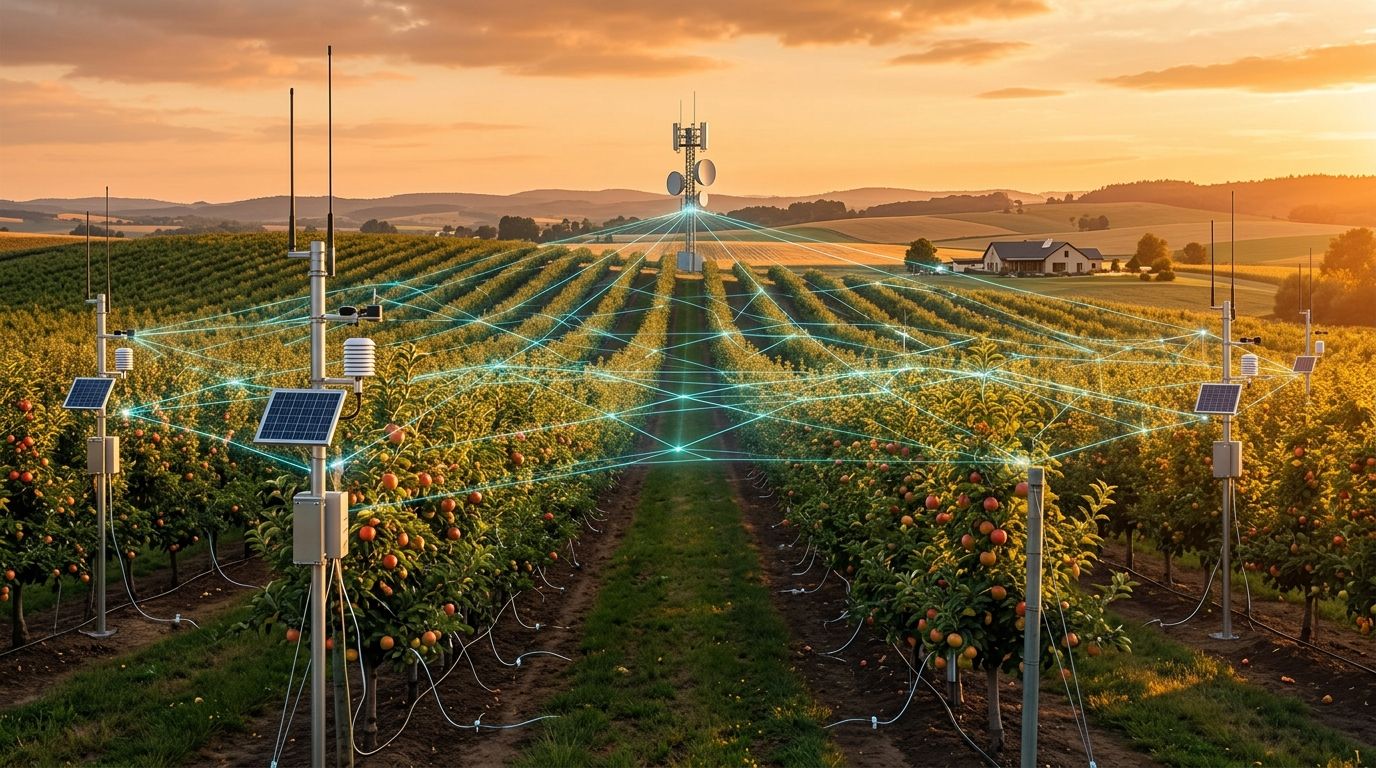
\includegraphics[width=0.92\textwidth]{figures/zigbee_farm_mesh_realistic.jpg}
    \caption{การติดตั้งโหนดโครงข่ายแบบเมช Zigbee 3.0 กระจายตัวในแปลงเกษตรกรรมและแปลงปลูกอัจฉริยะ}
    \label{fig:zigbee_farm_mesh}
\end{figure}

\section{สถาปัตยกรรมอุปกรณ์ตามมาตรฐาน Zigbee 3.0}

มาตรฐาน \textbf{ซิกบี 3.0 (Zigbee 3.0)}\index{Zigbee 3.0@Zigbee 3.0} ทำงานบนมาตรฐานชั้นกายภาพและชั้นควบคุมการเข้าถึงตัวกลาง IEEE 802.15.4\index{IEEE 802.15.4@IEEE 802.15.4} โดยผสานรวมมาตรฐานย่อยเดิม ได้แก่ Zigbee Home Automation, Zigbee Light Link และ Zigbee Building Automation เข้าไว้ด้วยกันภายใต้โปรไฟล์สากลหนึ่งเดียว ภายในเครือข่ายกำหนดบทบาทของอุปกรณ์ออกเป็น 3 ชนิด

\begin{protocolbox}[บทบาทและหน้าที่ของโหนดในเครือข่าย Zigbee 3.0]
โครงสร้างเครือข่ายแบ่งบทบาทของอุปกรณ์ตามการใช้พลังงานและหน้าที่ดังนี้
\begin{enumerate}
    \item \textbf{ตัวประสานงานเครือข่าย (Zigbee Coordinator หรือ ZC)}\index{Coordinator@Coordinator (ตัวประสานงาน)} เป็นโหนดหลักทำหน้าที่ริเริ่มเครือข่าย เลือกช่องสัญญาณความถี่ กำหนดค่าพารามิเตอร์ด้านความปลอดภัย จัดเก็บตารางการจัดเส้นทางระดับศูนย์กลาง และเชื่อมโยงสู่เกตเวย์ภายนอก ในเครือข่ายจะมี ZC ได้เพียง 1 ตัวเท่านั้น
    \item \textbf{เราเตอร์โครงข่าย (Zigbee Router หรือ ZR)}\index{Router@Router (เราเตอร์โครงข่าย)} ทำหน้าที่ส่งต่อแพ็กเก็ตข้อมูลระหว่างโหนด เป็นสะพานขยายระยะการส่งสัญญาณและทำหน้าที่รับคำขอเชื่อมต่อจากโหนดลูก อุปกรณ์เราเตอร์ต้องต่อไฟเลี้ยงตลอดเวลา
    \item \textbf{อุปกรณ์ปลายทาง (Zigbee End Device หรือ ZED)}\index{End Device@End Device (อุปกรณ์ปลายทาง)} เป็นโหนดตรวจวัดเซนเซอร์ที่ใช้พลังงานแบตเตอรี่ ไม่มีหน้าที่ส่งต่อข้อมูลให้โหนดอื่น และสามารถเข้าสู่โหมดประหยัดพลังงานระดับลึก (Deep Sleep) ได้นานหลายปี
\end{enumerate}
\end{protocolbox}

\begin{table}[H]
\caption{การเปรียบเทียบบทบาทและคุณลักษณะของโหนดในเครือข่าย Zigbee 3.0}
\label{tab:zigbee_device_roles}
\centering
\small
\begin{tabularx}{\textwidth}{p{3.2cm} >{\raggedright\arraybackslash}X >{\raggedright\arraybackslash}X c}
\toprule
\textbf{ชนิดอุปกรณ์} & \textbf{แหล่งจ่ายพลังงาน} & \textbf{บทบาทหลักในเครือข่าย} & \textbf{โหมดประหยัดไฟ} \\
\midrule
Coordinator (ZC) & ไฟฟ้ากระแสสลับต่อเนื่อง & ริเริ่มเครือข่าย, จัดการกุญแจความปลอดภัย & ไม่รองรับ \\
Router (ZR) & ไฟฟ้ากระแสสลับ หรือ โซลาร์ & ส่งต่อแพ็กเก็ตข้อมูล, ขยายรัศมีโครงข่าย & ไม่รองรับ \\
End Device (ZED) & แบตเตอรี่ Li-SOCl2 / LiFePO4 & อ่านค่าเซนเซอร์, ส่งข้อมูลขึ้นโหนดแม่ & รองรับ Deep Sleep \\
\bottomrule
\end{tabularx}
\end{table}

\section{อัลกอริทึมการจัดเส้นทางแบบเมชและการซ่อมแซมโครงข่ายด้วยตนเอง}

ความสามารถในการจัดเส้นทาง \textbf{การจัดเส้นทางแบบเมช (Mesh Routing)} ของ Zigbee อาศัยอัลกอริทึม AODV (Ad hoc On-Demand Distance Vector)\index{AODV Routing@AODV Routing (การจัดเส้นทาง)} ร่วมกับกลไกตารางเพื่อนบ้าน (Neighbor Table) เพื่อสร้างเส้นทางการส่งข้อมูลแบบหลายช่วง (Multi-hop) อัตโนมัติ

\begin{agribox}[กระบวนการค้นหาและซ่อมแซมเส้นทางอัตโนมัติ]
เมื่อโหนดเซนเซอร์ ZED หรือเราเตอร์ ZR ต้องการส่งข้อมูลไปยัง Coordinator กระบวนการทำงานเกิดขึ้นดังนี้
\begin{enumerate}
    \item \textbf{Route Request (RREQ)} โหนดต้นทางกระจายแพ็กเก็ตค้นหาเส้นทางไปยังเราเตอร์เพื่อนบ้านในระยะรัศมีคลื่นวิทยุ
    \item \textbf{Link Quality Assessment} เราเตอร์แต่ละตัวจะประเมินคุณภาพสัญญาณรับ (LQI) และค่าความแรงสัญญาณ (RSSI) เพื่อคำนวณต้นทุนการส่งผ่าน (Link Cost)
    \item \textbf{Route Reply (RREP)} โหนดปลายทางหรือเราเตอร์ที่มีเส้นทางสู่ปลายทาง จะส่งแพ็กเก็ตตอบกลับเพื่อยืนยันเส้นทางที่มีต้นทุนรวมต่ำที่สุด
    \item \textbf{Self-Healing Route Recovery}\index{Self-Healing@Self-Healing (การกู้คืนเครือข่าย)} หากเราเตอร์ตัวกลางหยุดทำงานเนื่องจากแบตเตอรี่หมดหรือถูกกีดขวาง โหนดต้นทางจะตรวจพบความล้มเหลวและเริ่มส่งแพ็กเก็ต RREQ ใหม่ เพื่อค้นหาเส้นทางสำรองรอบสิ่งกีดขวางภายในเวลาไม่กี่วินาที
\end{enumerate}
\end{agribox}

\section{การวิเคราะห์เปรียบเทียบระหว่าง Zigbee 3.0, LoRaWAN, Wi-Fi และ BLE}

ในการวางสถาปัตยกรรมระบบไอโอทีทางการเกษตร วิศวกรจำเป็นต้องเลือกเทคโนโลยีที่ตอบโจทย์ความต้องการของพื้นที่และปริมาณข้อมูลอย่างเหมาะสม\index{LoRaWAN@LoRaWAN} ตารางที่ \ref{tab:wireless_tech_comparison} สรุปเปรียบเทียบมาตรฐานสื่อสารสำคัญ

\begin{table}[H]
\caption{การวิเคราะห์เปรียบเทียบสมรรถนะเทคโนโลยีสื่อสารไร้สายในงานเกษตรกรรม}
\label{tab:wireless_tech_comparison}
\centering
\small
\begin{tabularx}{\textwidth}{p{2.6cm} c c c >{\raggedright\arraybackslash}X}
\toprule
\textbf{เทคโนโลยี} & \textbf{อัตราส่งข้อมูล} & \textbf{ระยะทางต่อช่วง} & \textbf{การใช้พลังงาน} & \textbf{จุดเด่นและความเหมาะสม} \\
\midrule
Zigbee 3.0 & 250 kbps & 30--100 m & ต่ำมาก (mA) & โครงข่ายเมชหลายโหนดหนาแน่น ค่า Latency ต่ำ \\
LoRaWAN & 0.3--50 kbps & 2--15 km & ต่ำมาก & โครงข่ายดาวระยะไกล เหมาะกับเซนเซอร์เดี่ยวห่างไกล \\
Wi-Fi (802.11b/g/n) & 11--150 Mbps & 50--100 m & สูง & แบนด์วิดท์สูง เหมาะสำหรับกล้องสตรีมภาพและวิดีโอ \\
BLE (Bluetooth 5) & 1--2 Mbps & 10--40 m & ต่ำมาก & ส่งข้อมูลระยะใกล้ เหมาะสำหรับการตั้งค่าหน้างาน \\
\bottomrule
\end{tabularx}
\end{table}

จากตารางข้างต้นจะเห็นได้ว่า สำหรับแปลงเกษตรกรรมแบบโรงเรือน แปลงผลไม้ที่มีการติดตั้งเซนเซอร์หนาแน่นหลายสิบโหนด และต้องการส่งข้อมูลแบบสองทิศทางเพื่อควบคุมวาล์วน้ำและสวิตช์อย่างทันท่วงที (Latency ไม่เกิน 100 มิลลิวินาที) เทคโนโลยี Zigbee 3.0 มีความได้เปรียบ LoRaWAN อย่างชัดเจนในแง่ของแบนด์วิดท์และความสามารถในการรับส่งคำสั่งควบคุม

\clearpage

% ------------------------------------------------------------
% คำถามทบทวนท้ายบทที่ 1
% ------------------------------------------------------------
\section*{คำถามทบทวนท้ายบทที่ 1}
\addcontentsline{toc}{section}{คำถามทบทวนท้ายบทที่ 1}

\begin{enumerate}
    \item จงอธิบายกลไกทางฟิสิกส์ที่ทำให้คลื่นความถี่ 2.4 GHz เกิดการสูญเสียกำลังส่งอย่างรวดเร็วเมื่อแพร่ผ่านทรงพุ่มแปลงผลไม้ พร้อมระบุตัวแปรสำคัญในแบบจำลองของฟิตซ์เจอรัลด์
    \item ในเครือข่าย Zigbee 3.0 เหตุใดจึงอนุญาตให้มี Coordinator ได้เพียง 1 ตัว และอุปกรณ์ชนิดใดบ้างที่สามารถทำหน้าที่ขยายรัศมีโครงข่ายแบบเมชได้
    \item อธิบายขั้นตอนการทำงานของอัลกอริทึม AODV เมื่อเกิดเหตุการณ์ที่เราเตอร์ตัวกลางหยุดทำงานกะทันหัน เครือข่ายมีกระบวนการซ่อมแซมเส้นทางด้วยตนเองอย่างไร
    \item จงเปรียบเทียบข้อดีและข้อจำกัดระหว่าง Zigbee 3.0 และ LoRaWAN ในการติดตั้งระบบน้ำอัจฉริยะที่ต้องการทั้งการอ่านค่าเซนเซอร์และการสั่งเปิดปิดโซลินอยด์วาล์ว 24 ตัว
    \item หากต้องการออกแบบเครือข่าย Zigbee สำหรับโรงเรือนอัจฉริยะขนาด 40 เมตรคูณ 100 เมตร จงระบุจำนวนและตำแหน่งที่เหมาะสมของ Coordinator, Router และ End Device เพื่อให้การเชื่อมต่อมีเสถียรภาพสูงสุด
\end{enumerate}

\clearpage


% บทที่ 2: ระบบนิเวศเซนเซอร์เกษตรและสะพานเชื่อมต่ออุตสาหกรรม RS485 Modbus
% ============================================================
% บทที่ 2: ระบบนิเวศเซนเซอร์เกษตรและสะพานเชื่อมต่ออุตสาหกรรม RS485 Modbus
% ============================================================
\chapter[ระบบนิเวศเซนเซอร์เกษตรและสะพานเชื่อมต่ออุตสาหกรรม RS485 Modbus]{ระบบนิเวศเซนเซอร์เกษตร\\และสะพานเชื่อมต่ออุตสาหกรรม RS485 Modbus}
\label{chap:ch02}

% ------------------------------------------------------------
% แผนบริหารการสอนประจำบทที่ 2 (หน้า 1/2)
% ------------------------------------------------------------
\section*{แผนบริหารการสอนประจำบทที่ 2}
\addcontentsline{toc}{section}{แผนบริหารการสอนประจำบทที่ 2}

\begin{planbox}{หัวข้อเนื้อหาประจำบท}
\begin{enumerate}[topsep=1pt, itemsep=0.5pt, partopsep=0pt, parsep=0pt, leftmargin=1.5em]
    \item สรีรวิทยาของพืชและการตรวจวัดสภาพแวดล้อมทางฟิสิกส์ในดินและบรรยากาศ
    \item เซนเซอร์ตรวจวัดดินแบบหลายพารามิเตอร์ ความชื้น อุณหภูมิ การนำไฟฟ้า และธาตุอาหาร NPK
    \item การตรวจวัดสภาวะภูมิอากาศจุลภาค อุณหภูมิ ความชื้นสัมพัทธ์ และรังสีสังเคราะห์แสง PAR
    \item สถาปัตยกรรมสะพานสื่อสารเชื่อมต่อมาตรฐานอุตสาหกรรม RS485 Modbus RTU สู่ Zigbee
    \item การวิเคราะห์เปรียบเทียบระหว่างโหนดเซนเซอร์เชิงพาณิชย์และฮาร์ดแวร์โอเพนซอร์สแบบกำหนดเอง
\end{enumerate}
\end{planbox}

\begin{planbox}{วัตถุประสงค์เชิงพฤติกรรม}
\begin{enumerate}[topsep=1pt, itemsep=0.5pt, partopsep=0pt, parsep=0pt, leftmargin=1.5em]
    \item อธิบายหลักการทำงานของหัววัดความชื้นดินแบบความจุไฟฟ้าและการนำไฟฟ้าได้อย่างถูกต้อง
    \item เชื่อมต่อและสื่อสารกับเซนเซอร์อุตสาหกรรมผ่านโพรโทคอล Modbus RTU ได้อย่างสมบูรณ์
    \item ออกแบบวงจรสะพานสื่อสาร RS485 ร่วมกับโมดูลไมโครคอนโทรลเลอร์ Zigbee ได้
    \item คำนวณและปรับเทียบค่าความถูกต้องของข้อมูลเซนเซอร์ทางการเกษตรได้อย่างเป็นระบบ
    \item ประเมินความคุ้มค่าและความเหมาะสมระหว่างการจัดซื้ออุปกรณ์สำเร็จรูปและการพัฒนาขึ้นเองได้
\end{enumerate}
\end{planbox}

\newpage

% ------------------------------------------------------------
% แผนบริหารการสอนประจำบทที่ 2 (หน้า 2/2)
% ------------------------------------------------------------
\begin{planbox}{วิธีสอนและกิจกรรมการเรียนการสอน}
\begin{enumerate}[topsep=1pt, itemsep=0.5pt, partopsep=0pt, parsep=0pt, leftmargin=1.5em]
    \item การบรรยายหลักการฟิสิกส์ของหัววัดเซนเซอร์ดินและเซนเซอร์ทางแสง
    \item การสาธิตการต่อวงจรและส่งคำสั่งอ่านค่ารีจิสเตอร์ Modbus RTU ด้วยโปรแกรมทดสอบ
    \item การฝึกปฏิบัติการต่อสายโพรบ 7-in-1 ร่วมกับไอซีแปลงสัญญาณ MAX485 และโหนด Zigbee
    \item การทดลองปรับเทียบค่า EC และ pH ด้วยสารละลายมาตรฐานในห้องปฏิบัติการ
    \item การอภิปรายเปรียบเทียบคุณสมบัติเชิงเทคนิคและงบประมาณการลงทุนในแปลงจริง
\end{enumerate}
\end{planbox}

\begin{planbox}{สื่อการเรียนการสอน}
\begin{enumerate}[topsep=1pt, itemsep=0.5pt, partopsep=0pt, parsep=0pt, leftmargin=1.5em]
    \item เอกสารประกอบการสอนวิชาระบบเซนเซอร์และเครื่องมือวัดทางการเกษตร
    \item หัววัดเซนเซอร์ดินอุตสาหกรรม RS485 ชนิด 7-in-1 โพรบสแตนเลสสตีลมาตรฐาน IP68
    \item เซนเซอร์อุณหภูมิและความชื้น SHT30 หัวครอบโลหะเผา และเซนเซอร์วัดแสง BH1750
    \item โมดูลแปลงระดับสัญญาณ TTL เป็น RS485 พร้อมวงจรแยกสัญญาณกัลวานิก
    \item สารละลายมาตรฐานสำหรับการปรับเทียบค่าการนำไฟฟ้าและกรดด่าง
\end{enumerate}
\end{planbox}

\begin{planbox}{การวัดและประเมินผล}
\begin{enumerate}[topsep=1pt, itemsep=0.5pt, partopsep=0pt, parsep=0pt, leftmargin=1.5em]
    \item การประเมินผลการทดสอบภาคความรู้ด้านการคำนวณและหลักการทำงานของเซนเซอร์
    \item การตรวจผลงานการต่อวงจรสะพานสื่อสาร RS485 และความถูกต้องในการอ่านรีจิสเตอร์
    \item การประเมินความแม่นยำในการปรับเทียบค่าเซนเซอร์ตามขั้นตอนมาตรฐาน
    \item การมีส่วนร่วมและความปลอดภัยในการใช้อุปกรณ์วัดทางไฟฟ้าในห้องปฏิบัติการ
\end{enumerate}
\end{planbox}

\clearpage

% ------------------------------------------------------------
% เนื้อหาบทที่ 2
% ------------------------------------------------------------
\section{การตรวจวัดสภาพแวดล้อมทางฟิสิกส์ในดินสำหรับการเกษตรแม่นยำ}

การจัดการน้ำและธาตุอาหารพืชอย่างมีประสิทธิภาพ \textbf{การตรวจวัดสภาวะของดิน (Soil Environmental Sensing)}\index{Soil Sensing@Soil Sensing (การตรวจวัดสภาพดิน)} มีความสำคัญยิ่งต่อการเจริญเติบโตของรากพืช ดินที่มีความชื้นเหมาะสมและการนำไฟฟ้า (Electrical Conductivity หรือ EC)\index{EC@EC (Electrical Conductivity)} ที่สมดุลจะช่วยให้พืชดูดซึมสารอาหารได้อย่างเต็มที่

เซนเซอร์ดินมาตรฐานอุตสาหกรรมในปัจจุบันนิยมใช้โพรบแบบแท่งเข็มสแตนเลสเกรด 316L ทนต่อการกัดกร่อนจากสารเคมีและปุ๋ย โดยทำงานร่วมกันหลายระบบในหัววัดเดียว ดังนี้

\begin{agribox}[พารามิเตอร์สำคัญของหัววัดดินอุตสาหกรรม]
หัววัดดินสมัยใหม่สามารถตรวจวัดข้อมูลได้พร้อมกันถึง 7 พารามิเตอร์
\begin{enumerate}
    \item \textbf{ความชื้นในดินเชิงปริมาตร (Volumetric Water Content หรือ VWC)}\index{VWC@VWC (ความชื้นดินเชิงปริมาตร)} ใช้หลักการวัดความจุไฟฟ้าความถี่สูง (Frequency Domain Reflectometry หรือ FDR)\index{FDR@FDR (Frequency Domain Reflectometry)} ที่ช่วงความถี่ 50--100 MHz เพื่อลดอิทธิพลของเกลือแร่ในดิน
    \item \textbf{อุณหภูมิดิน (Soil Temperature)} วัดด้วยความต้านทานไวต่ออุณหภูมิ (RTD หรือ NTC ความแม่นยำสูง) สำหรับนำไปชดเชยค่าความคลาดเคลื่อนของการนำไฟฟ้า
    \item \textbf{การนำไฟฟ้าในดิน (Electrical Conductivity หรือ EC)} วัดความสามารถในการนำกระแสไฟฟ้ากระแสสลับความถี่สูงระหว่างขั้วอิเล็กโทรดเพื่อประเมินระดับความเข้มข้นของเกลือแร่
    \item \textbf{ความเป็นกรดด่าง (Soil pH)}\index{Soil pH@Soil pH (ความเป็นกรดด่างในดิน)} วัดศักย์ไฟฟ้าเคมีเปรียบเทียบกับขั้วอ้างอิง
    \item \textbf{ธาตุอาหารหลัก (Nitrogen, Phosphorus, Potassium หรือ NPK)}\index{NPK@NPK (ธาตุอาหารหลัก)} ตรวจวัดการดูดกลืนแสงและปฏิกิริยาเคมีไฟฟ้าเชิงอนุมาน
\end{enumerate}
\end{agribox}

\begin{figure}[H]
    \centering
    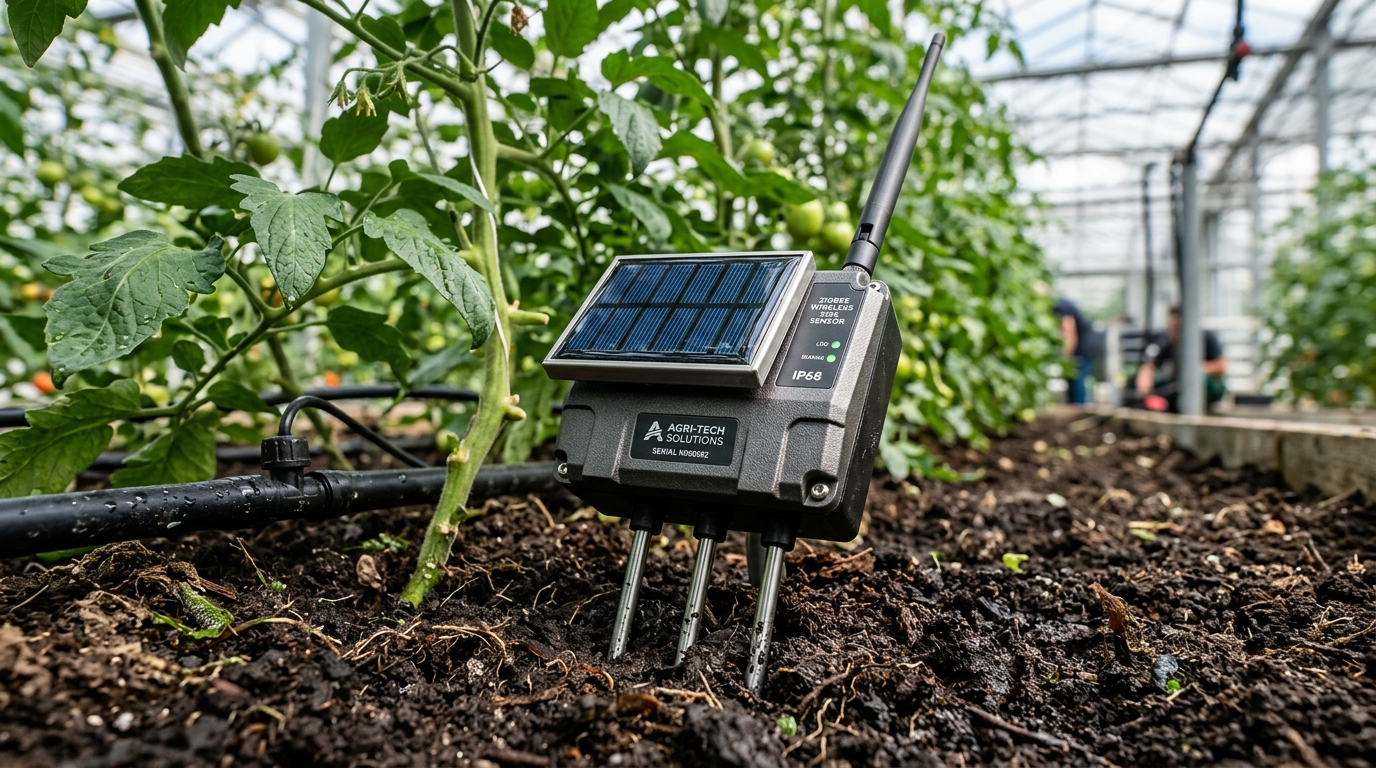
\includegraphics[width=0.88\textwidth]{figures/zigbee_soil_sensor_realistic.jpg}
    \caption{การติดตั้งหัววัดเซนเซอร์ดินอุตสาหกรรมแบบฝังลึกในแปลงเกษตรพร้อมโหนดรับส่งข้อมูล Zigbee}
    \label{fig:zigbee_soil_sensor}
\end{figure}

\section{การตรวจวัดสภาวะบรรยากาศและรังสีดวงอาทิตย์}

นอกเหนือจากสภาวะใต้ดินแล้ว สภาวะบรรยากาศเหนือดินมีอิทธิพลโดยตรงต่อกระบวนการสังเคราะห์ด้วยแสงและการคายน้ำของพืช การตรวจวัด \textbf{ความดันไอขาดดุล (Vapor Pressure Deficit หรือ VPD)}\index{VPD@VPD (ความดันไอขาดดุล)} ซึ่งคำนวณจากอุณหภูมิอากาศและความชื้นสัมพัทธ์ ถือเป็นตัวชี้วัดสำคัญที่สุดในการตัดสินใจเปิดปิดระบบพ่นหมอกและพัดลมระบายอากาศในโรงเรือน

ค่าความดันไอขาดดุลสามารถคำนวณได้จากสมการของเตเทนส์ (Tetens Equation)
\begin{equation}
    e_s(T) = 0.61078 \exp\left( \frac{17.27 T}{T + 237.3} \right) \quad \text{[kPa]}
\end{equation}
\begin{equation}
    \text{VPD} = e_s(T) \times \left(1 - \frac{\text{RH}}{100}\right) \quad \text{[kPa]}
\end{equation}
โดยที่ $e_s(T)$ คือความดันไออิ่มตัวที่อุณหภูมิ $T$ ในหน่วยองศาเซลเซียส และ $\text{RH}$ คือความชื้นสัมพัทธ์ในหน่วยเปอร์เซ็นต์

\begin{figure}[H]
    \centering
    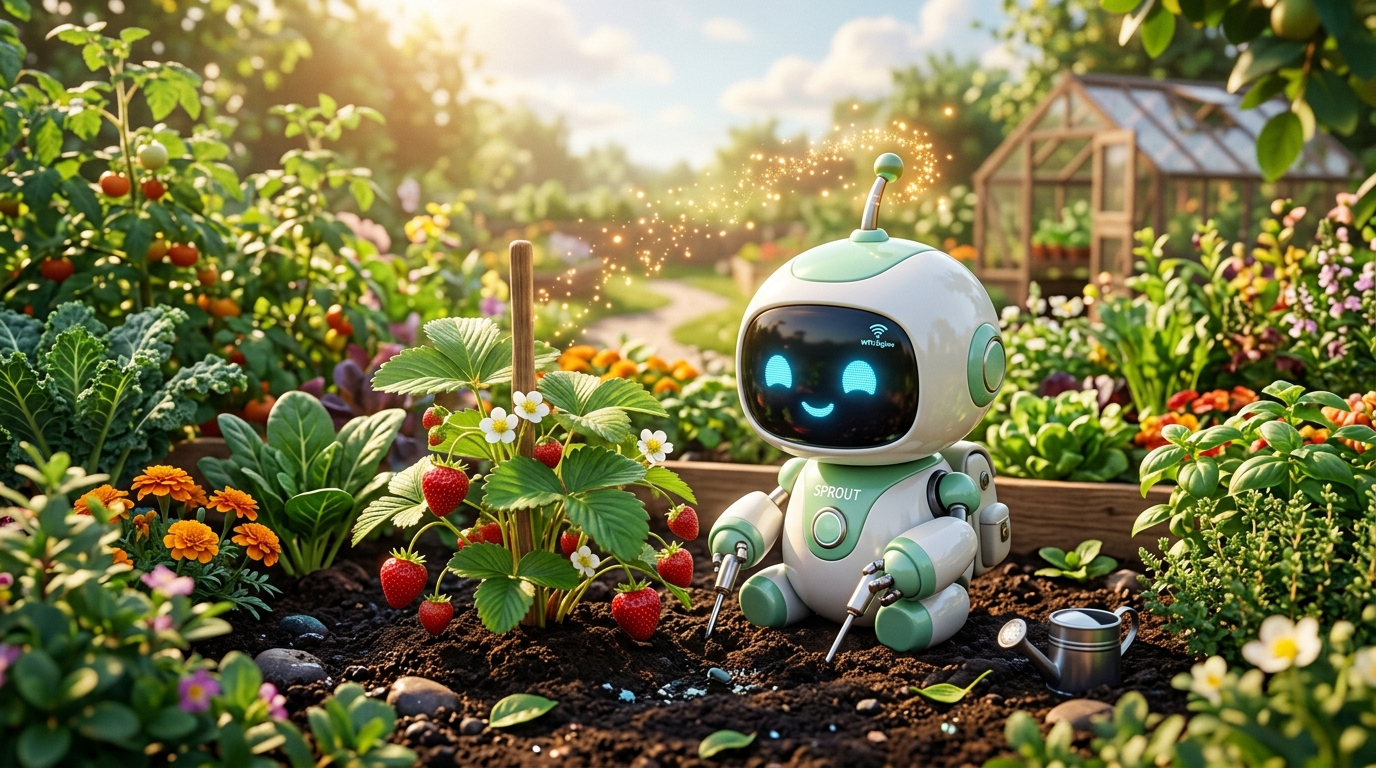
\includegraphics[width=0.88\textwidth]{figures/zigbee_sensor_pixar_3d.jpg}
    \caption{แบบจำลอง 3 มิติแสดงโครงสร้างสถาปัตยกรรมโหนดเซนเซอร์ Zigbee บูรณาการหัววัดดินและหัววัดสภาพอากาศ}
    \label{fig:zigbee_sensor_3d}
\end{figure}

\section{สถาปัตยกรรมสะพานสื่อสาร RS485 Modbus RTU สู่ Zigbee}

เนื่องจากเซนเซอร์ภาคสนามเกรดอุตสาหกรรมส่วนใหญ่ใช้พอร์ตสื่อสารแบบสายชนิด \textbf{อาร์เอส-485 (RS485)}\index{RS485@RS485} และโพรโทคอล \textbf{มอดบัส (Modbus RTU)}\index{Modbus RTU@Modbus RTU} เพื่อความทนทานต่อสัญญาณรบกวนแม่เหล็กไฟฟ้า การนำข้อมูลเข้าสู่โครงข่ายไร้สาย Zigbee จึงต้องอาศัยอุปกรณ์สะพานสื่อสาร (Bridge Node)

\begin{protocolbox}[โครงสร้างคำสั่งและการตรวจสอบความถูกต้องของ Modbus RTU]
การติดต่อสื่อสารแบบ Modbus RTU ทำงานในรูปแบบ Master-Slave โดยโหนด Zigbee จะทำหน้าที่เป็น Master ส่งคำสั่งแบบไบนารีไปยังเซนเซอร์โครงสร้างเฟรมประกอบด้วย
\begin{enumerate}
    \item \textbf{Slave Address (1 ไบต์)} ที่อยู่ประจำอุปกรณ์ เช่น 0x01
    \item \textbf{Function Code (1 ไบต์)} ฟังก์ชันการทำงาน เช่น 0x03 (Read Holding Registers)
    \item \textbf{Starting Address (2 ไบต์)} แอดเดรสเริ่มต้นของรีจิสเตอร์ที่ต้องการอ่าน
    \item \textbf{Number of Points (2 ไบต์)} จำนวนรีจิสเตอร์ที่ต้องการอ่าน เช่น 0x0007 (อ่าน 7 ตัว)
    \item \textbf{Cyclic Redundancy Check หรือ CRC-16 (2 ไบต์)} รหัสตรวจสอบความถูกต้องข้อมูลตามพหุนาม $x^{16} + x^{15} + x^2 + 1$
\end{enumerate}
\end{protocolbox}

\begin{table}[H]
\caption{ตัวอย่างผังรีจิสเตอร์ของหัววัดดินอุตสาหกรรม 7-in-1 Modbus RTU}
\label{tab:modbus_register_map}
\centering
\small
\begin{tabularx}{\textwidth}{c c c >{\raggedright\arraybackslash}X c}
\toprule
\textbf{Register Address} & \textbf{พารามิเตอร์} & \textbf{หน่วย} & \textbf{ตัวคูณสเกล (Scaling Factor)} & \textbf{ชนิดข้อมูล} \\
\midrule
0x0000 & ความชื้นดิน (Soil Moisture) & \% & 0.1 (เช่น ค่า 452 หมายถึง 45.2\%) & 16-bit Unsigned \\
0x0001 & อุณหภูมิดิน (Soil Temp) & $^\circ\text{C}$ & 0.1 (ค่าลบใช้ 2's Complement) & 16-bit Signed \\
0x0002 & การนำไฟฟ้า (Soil EC) & $\mu\text{S/cm}$ & 1 (เช่น ค่า 1250 หมายถึง 1250 $\mu\text{S/cm}$) & 16-bit Unsigned \\
0x0003 & ความเป็นกรดด่าง (Soil pH) & pH & 0.1 (เช่น ค่า 68 หมายถึง 6.8 pH) & 16-bit Unsigned \\
0x0004 & ไนโตรเจน (Nitrogen - N) & mg/kg & 1 & 16-bit Unsigned \\
0x0005 & ฟอสฟอรัส (Phosphorus - P) & mg/kg & 1 & 16-bit Unsigned \\
0x0006 & โพแทสเซียม (Potassium - K) & mg/kg & 1 & 16-bit Unsigned \\
\bottomrule
\end{tabularx}
\end{table}

\begin{warningbox}[ข้อควรระวังในการต่อวงจร RS485 ภาคสนาม]
การติดตั้งสายสัญญาณ RS485 ในแปลงเกษตรกรรมมีความเสี่ยงสูงต่อฟ้าผ่าและแรงดันเกินชั่วขณะ (Transient Voltage) วิศวกรต้องปฏิบัติตามข้อกำหนดดังนี้
\begin{enumerate}
    \item ใช้สายสัญญาณชนิดคู่บิดเกลียวพร้อมแผ่นชิลด์กันสัญญาณกวน (Shielded Twisted Pair หรือ STP) โดยต่อกราวด์แผ่นชิลด์ที่ฝั่งเกตเวย์เพียงจุดเดียว (Single-Point Grounding) เพื่อป้องกัน Ground Loop
    \item ติดตั้งตัวต้านทานต่อปลายสาย (Termination Resistor) ขนาด 120 โอห์ม ที่จุดปลายสุดของสายสัญญาณทั้งสองด้าน เพื่อป้องกันการสะท้อนของคลื่น
    \item ติดตั้งไดโอดป้องกันแรงดันเสิร์จ (TVS Diode) และวงจรตัดต่อกัลวานิก (Optocoupler / Digital Isolator) เพื่อป้องกันไม่ให้ไฟกระชากทำลายบอร์ดไมโครคอนโทรลเลอร์
\end{enumerate}
\end{warningbox}

\section{การเปรียบเทียบระหว่างโหนดสำเร็จรูปเชิงพาณิชย์และโหนดโอเพนซอร์ส}

\begin{table}[H]
\caption{การวิเคราะห์เปรียบเทียบโหนดเซนเซอร์สำเร็จรูปเชิงพาณิชย์และโหนดโอเพนซอร์ส}
\label{tab:commercial_vs_custom}
\centering
\small
\begin{tabularx}{\textwidth}{p{3.0cm} >{\raggedright\arraybackslash}X >{\raggedright\arraybackslash}X}
\toprule
\textbf{หัวข้อเปรียบเทียบ} & \textbf{โหนดสำเร็จรูปเชิงพาณิชย์ (Commercial)} & \textbf{โหนดปรับแต่งเอง (Custom ESP32-C6)} \\
\midrule
ความง่ายในการใช้งาน & เสียบใช้งานได้ทันที ผูกกับแอปพลิเคชันสำเร็จรูป & ต้องเขียนเฟิร์มแวร์และออกแบบวงจรพิมพ์ \\
ความยืดหยุ่น & ปรับแต่งแก้ไขโพรโทคอลไม่ได้ & ปรับอัลกอริทึมและเพิ่มเซนเซอร์ได้อิสระ \\
การผสานรวมระบบ & มักติดล็อกอยู่กับเซิร์ฟเวอร์ผู้ผลิต (Vendor Lock-in) & เปิดกว้าง เชื่อมต่อตรงสู่ MQTT / Home Assistant \\
ต้นทุนต่อหน่วย & ราคาสูง (3,500--8,000 บาทต่อชุด) & ราคาต่ำ (800--1,800 บาทต่อชุด) \\
การบำรุงรักษา & ต้องส่งศูนย์บริการซ่อม & วิศวกรประจำฟาร์มสามารถเปลี่ยนอะไหล่ได้ทันที \\
\bottomrule
\end{tabularx}
\end{table}

\clearpage

% ------------------------------------------------------------
% คำถามทบทวนท้ายบทที่ 2
% ------------------------------------------------------------
\section*{คำถามทบทวนท้ายบทที่ 2}
\addcontentsline{toc}{section}{คำถามทบทวนท้ายบทที่ 2}

\begin{enumerate}
    \item จงอธิบายความแตกต่างระหว่างการวัดความชื้นดินแบบ Frequency Domain Reflectometry (FDR) และ Time Domain Reflectometry (TDR) เหตุใดวิธี FDR จึงเป็นที่นิยมในโหนดเซนเซอร์ขนาดเล็ก
    \item ค่าความดันไอขาดดุล (Vapor Pressure Deficit หรือ VPD) มีความสัมพันธ์กับอัตราการคายน้ำของพืชอย่างไร และเหตุใดการวัดเพียงค่าอุณหภูมิและความชื้นสัมพัทธ์แยกกันจึงไม่เพียงพอต่อการควบคุมโรงเรือนอัจฉริยะ
    \item กำหนดให้เซนเซอร์ดิน Modbus RTU ส่งข้อมูลไบนารีค่าความชื้น 0x01B8 และอุณหภูมิ 0x0104 จงคำนวณค่าจริงในหน่วยเปอร์เซ็นต์และองศาเซลเซียสตามผังรีจิสเตอร์ในตารางที่ \ref{tab:modbus_register_map}
    \item เหตุใดการต่อสายสัญญาณ RS485 ในระยะทางไกลจึงจำเป็นต้องติดตั้งตัวต้านทาน 120 โอห์มที่ปลายสาย หากไม่ติดตั้งจะส่งผลกระทบต่อรูปสัญญาณอย่างไร
    \item ในการออกแบบโหนดเซนเซอร์ดินที่ติดตั้งกลางแจ้ง จงอธิบายมาตรการป้องกันความชื้นและฝุ่นละอองตามมาตรฐาน IP68 และการป้องกันแรงดันกระชากจากฟ้าผ่า
\end{enumerate}

\clearpage


% บทที่ 3: เกตเวย์โครงข่ายและการบูรณาการระบบอัตโนมัติ Zigbee2MQTT
% ============================================================
% บทที่ 3: เกตเวย์โครงข่ายและการบูรณาการระบบอัตโนมัติ Zigbee2MQTT
% ============================================================
\chapter[เกตเวย์โครงข่ายและการบูรณาการระบบอัตโนมัติ Zigbee2MQTT]{เกตเวย์โครงข่าย\\และการบูรณาการระบบอัตโนมัติ Zigbee2MQTT}
\label{chap:ch03}

% ------------------------------------------------------------
% แผนบริหารการสอนประจำบทที่ 3 (หน้า 1/2)
% ------------------------------------------------------------
\section*{แผนบริหารการสอนประจำบทที่ 3}
\addcontentsline{toc}{section}{แผนบริหารการสอนประจำบทที่ 3}

\begin{planbox}{หัวข้อเนื้อหาประจำบท}
\begin{enumerate}[topsep=1pt, itemsep=0.5pt, partopsep=0pt, parsep=0pt, leftmargin=1.5em]
    \item สถาปัตยกรรมตัวประสานงานโครงข่ายฮาร์ดแวร์ CC2652P และ EFR32MG21
    \item สถาปัตยกรรมซอฟต์แวร์สะพานข้อมูล Zigbee2MQTT และการบริหารจัดการเครือข่าย
    \item โครงสร้างหัวข้อข้อมูล MQTT และข้อกำหนดโครงสร้างเพย์โหลดแบบ JSON Telemetry
    \item การเชื่อมโยงข้อมูลสู่แพลตฟอร์มบริหารจัดการฟาร์มอัจฉริยะ Home Assistant และ Node-RED
    \item ความปลอดภัยของเครือข่าย กุญแจรหัสผ่าน และการป้องกันการแทรกแซงสัญญาณ
\end{enumerate}
\end{planbox}

\begin{planbox}{วัตถุประสงค์เชิงพฤติกรรม}
\begin{enumerate}[topsep=1pt, itemsep=0.5pt, partopsep=0pt, parsep=0pt, leftmargin=1.5em]
    \item ติดตั้งและตั้งค่าเฟิร์มแวร์ตัวประสานงาน CC2652P ได้อย่างถูกต้อง
    \item กำหนดค่าคอนฟิกูเรชันของโปรแกรม Zigbee2MQTT ให้สื่อสารกับโหนดในฟาร์มได้
    \item ออกแบบผังโครงสร้างหัวข้อ MQTT สำหรับข้อมูลโทรมาตรและคำสั่งควบคุมได้อย่างมีมาตรฐาน
    \item สร้างระบบอัตโนมัติเปิดปิดวาล์วน้ำตามเงื่อนไขของเซนเซอร์ใน Home Assistant ได้
    \item กำหนดค่าความปลอดภัยและการเข้ารหัส AES-128 บนเครือข่าย Zigbee ได้อย่างรัดกุม
\end{enumerate}
\end{planbox}

\newpage

% ------------------------------------------------------------
% แผนบริหารการสอนประจำบทที่ 3 (หน้า 2/2)
% ------------------------------------------------------------
\begin{planbox}{วิธีสอนและกิจกรรมการเรียนการสอน}
\begin{enumerate}[topsep=1pt, itemsep=0.5pt, partopsep=0pt, parsep=0pt, leftmargin=1.5em]
    \item การบรรยายหลักการทำงานของเกตเวย์และการแปลงโพรโทคอลระดับบริดจ์
    \item การสาธิตการแฟลชเฟิร์มแวร์ Z-Stack และการตั้งค่า Zigbee2MQTT บน Raspberry Pi
    \item การทดลองจับคู่โหนดเซนเซอร์ใหม่เข้าสู่โครงข่ายและการตรวจสอบแดชบอร์ดผังเมช
    \item การฝึกปฏิบัติการเขียน Automation Script สั่งงานรีเลย์ควบคุมน้ำใน Node-RED
    \item การทดสอบจำลองเหตุการณ์ขาดการเชื่อมต่ออินเทอร์เน็ตเพื่อประเมินเสถียรภาพระดับโลคอล
\end{enumerate}
\end{planbox}

\begin{planbox}{สื่อการเรียนการสอน}
\begin{enumerate}[topsep=1pt, itemsep=0.5pt, partopsep=0pt, parsep=0pt, leftmargin=1.5em]
    \item บอร์ดคอมพิวเตอร์แม่ข่าย Raspberry Pi 4 หรือ Single Board Computer
    \item ตัวประสานงาน USB Zigbee 3.0 Coordinator (ชิปเซต TI CC2652P) พร้อมเสา 5dBi
    \item ซอฟต์แวร์ Zigbee2MQTT, Eclipse Mosquitto MQTT Broker และ Home Assistant OS
    \item โปรแกรมเครื่องมือทดสอบ MQTT Explorer สำหรับตรวจสอบข้อความ JSON
    \item ผังโครงสร้างเครือข่ายและสเปกการตั้งค่าพารามิเตอร์ด้านความปลอดภัย
\end{enumerate}
\end{planbox}

\begin{planbox}{การวัดและประเมินผล}
\begin{enumerate}[topsep=1pt, itemsep=0.5pt, partopsep=0pt, parsep=0pt, leftmargin=1.5em]
    \item การประเมินผลการติดตั้งและตั้งค่าเกตเวย์ให้สามารถจับคู่อุปกรณ์ได้อย่างสมบูรณ์
    \item การตรวจความถูกต้องของโครงสร้าง JSON Telemetry Payload ที่ส่งขึ้น MQTT Broker
    \item การประเมินผลการทำงานของระบบอัตโนมัติในการสั่งงานอุปกรณ์ขับโหลด
    \item การทดสอบความเข้าใจเกี่ยวกับกลไกความปลอดภัยและการเข้ารหัสข้อมูลในโครงข่าย
\end{enumerate}
\end{planbox}

\clearpage

% ------------------------------------------------------------
% เนื้อหาบทที่ 3
% ------------------------------------------------------------
\section{สถาปัตยกรรมฮาร์ดแวร์ตัวประสานงานเครือข่าย}

หัวใจสำคัญของการควบคุมและบริหารจัดการโครงข่าย Zigbee คือ \textbf{ตัวประสานงานโครงข่าย (Zigbee Coordinator)}\index{Coordinator@Coordinator (ตัวประสานงาน)} ซึ่งทำหน้าที่เป็นสะพานเชื่อมต่อระหว่างคลื่นวิทยุ IEEE 802.15.4 เข้ากับระบบเครือข่ายคอมพิวเตอร์ไอพี (Ethernet / Wi-Fi) ชิปเซตที่ได้รับการยอมรับในระดับอุตสาหกรรมสูงสุดในปัจจุบัน ได้แก่

\begin{protocolbox}[การเลือกชิปเซตสำหรับเกตเวย์เกษตรกรรม]
คุณลักษณะเชิงเปรียบเทียบของชิปเซต Coordinator
\begin{enumerate}
    \item \textbf{Texas Instruments CC2652P}\index{CC2652P@CC2652P (ชิปเซตตัวประสานงาน)} ไมโครคอนโทรลเลอร์แกน ARM Cortex-M4F พร้อมภาคขยายกำลังส่งในตัว (Power Amplifier หรือ PA) ให้กำลังส่งสูงสุดถึง $+20$ dBm รองรับการเชื่อมต่อโหนดโดยตรงได้มากกว่า 100 โหนด และรองรับโครงข่ายเมชรวมมากกว่า 200 โหนด มีเสถียรภาพสูงสุดกับระบบ Z-Stack
    \item \textbf{Silicon Labs EFR32MG21}\index{EFR32MG21@EFR32MG21} สถาปัตยกรรม ARM Cortex-M33 กำลังส่ง $+20$ dBm มีจุดเด่นด้านประสิทธิภาพการประมวลผลและการรองรับโพรโทคอล Thread และ Matter ในอนาคต
\end{enumerate}
\end{protocolbox}

สำหรับสภาพแวดล้อมฟาร์มเกษตรกรรม แนะนำให้ใช้ตัวประสานงานแบบเชื่อมต่อผ่านสายแลนพร้อมระบบจ่ายไฟผ่านสายสัญญาณ (Power over Ethernet หรือ PoE) มากกว่าแบบต่อตรงผ่านพอร์ต USB เข้ากับคอมพิวเตอร์ เนื่องจากสามารถติดตั้งเกตเวย์ไว้ในตำแหน่งเสาสูงกึ่งกลางแปลงปลูกเพื่อรับสัญญาณรอบทิศทางได้ดีที่สุด และลดสัญญาณรบกวนความถี่สูงจากพอร์ต USB 3.0

\begin{figure}[H]
    \centering
    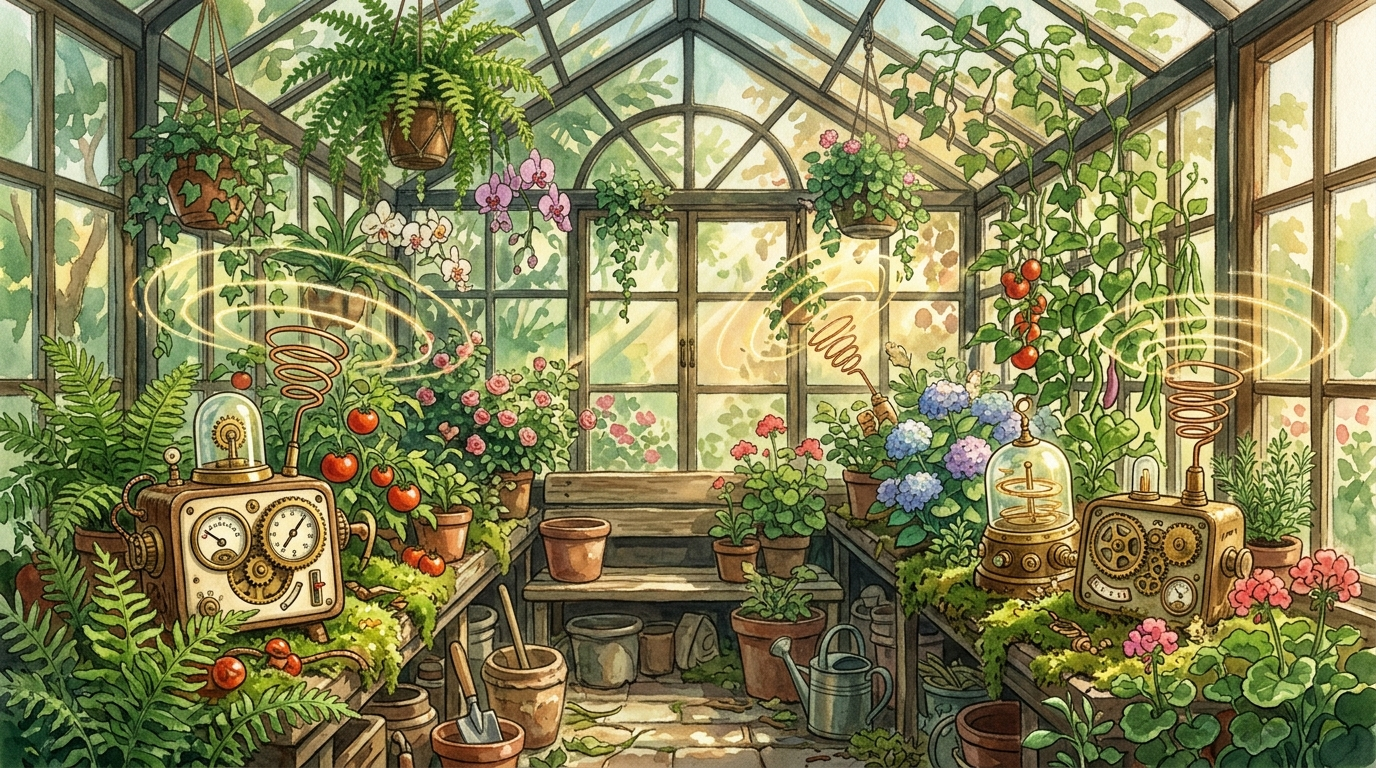
\includegraphics[width=0.90\textwidth]{figures/zigbee_greenhouse_ghibli.jpg}
    \caption{ระบบควบคุมอัตโนมัติภายในโรงเรือนเกษตรกรรมอัจฉริยะที่บูรณาการเกตเวย์ Zigbee และเซนเซอร์สิ่งแวดล้อม}
    \label{fig:zigbee_greenhouse}
\end{figure}

\section{สถาปัตยกรรมซอฟต์แวร์ Zigbee2MQTT}

โปรแกรม \textbf{ซิกบีทูเอ็มคิวทีที (Zigbee2MQTT)}\index{Zigbee2MQTT@Zigbee2MQTT} เป็นสะพานซอฟต์แวร์โอเพนซอร์สที่ทำหน้าที่แปลชุดข้อมูลและคำสั่งจากเฟรม ZCL (Zigbee Cluster Library)\index{ZCL@ZCL (Zigbee Cluster Library)} บนคลื่นวิทยุ ให้กลายเป็นข้อความ JSON บนโพรโทคอล MQTT\index{MQTT@MQTT} โดยตรง ทำให้ระบบไอโอทีสามารถสื่อสารกับอุปกรณ์ Zigbee จากผู้ผลิตต่างยี่ห้อกันได้มากกว่า 3,000 รุ่นอย่างไร้รอยต่อ

\begin{codebox}[ตัวอย่างไฟล์คอนฟิกูเรชัน configuration.yaml ของ Zigbee2MQTT]{yaml}
# Zigbee2MQTT configuration for smart farm
homeassistant: true
permit_join: false # Disabled after pairing for security

mqtt:
  base_topic: cmu_aiot/zigbee
  server: mqtt://10.0.0.1:1883
  user: farm_admin
  password: secure_farm_password_2027

serial:
  port: /dev/ttyUSB0
  adapter: zstack
  baudrate: 115200

advanced:
  pan_id: 0x1a62
  channel: 25 # Channel 25 avoids Wi-Fi channel 1, 6, 11 interference
  network_key:
    - 0x01
    - 0x03
    - 0x05
    - 0x07
    - 0x09
    - 0x0B
    - 0x0D
    - 0x0F
    - 0x02
    - 0x04
    - 0x06
    - 0x08
    - 0x0A
    - 0x0C
    - 0x0E
    - 0x10
\end{codebox}

\section{ข้อกำหนดหัวข้อและโครงสร้างข้อมูล JSON Telemetry}

การกำหนดโครงสร้าง \textbf{หัวข้อข้อมูล (MQTT Topics)} และเพย์โหลด ต้องสอดคล้องกับมาตรฐานการจัดการข้อมูลไอโอที เพื่อให้ระบบแสดงผล แดชบอร์ด และฐานข้อมูล Time-Series สามารถสืบค้นข้อมูลได้อย่างรวดเร็ว

\begin{protocolbox}[มาตรฐานโครงสร้าง MQTT Topic สำหรับฟาร์มเกษตรแม่นยำ]
โครงสร้างหัวข้อแบ่งออกเป็น 3 ระดับหลัก
\begin{enumerate}
    \item \textbf{Telemetry Stream} ส่งข้อมูลพารามิเตอร์เซนเซอร์จากโหนดขึ้นสู่โบรกเกอร์
    \begin{quote}
        \texttt{cmu\_aiot/zigbee/zone1/greenhouseA/soil\_node\_01}
    \end{quote}
    \item \textbf{Command Topic} รับคำสั่งจากระบบอัตโนมัติไปยังอุปกรณ์ขับโหลด (Actuator)
    \begin{quote}
        \texttt{cmu\_aiot/zigbee/zone1/greenhouseA/valve\_01/set}
    \end{quote}
    \item \textbf{Device State Topic} รายงานสถานะปัจจุบันของอุปกรณ์ขับโหลด
    \begin{quote}
        \texttt{cmu\_aiot/zigbee/zone1/greenhouseA/valve\_01}
    \end{quote}
\end{enumerate}
\end{protocolbox}

\begin{codebox}[ตัวอย่างเพย์โหลด JSON Telemetry จากโหนดตรวจวัดสภาพดินและบรรยากาศ]{json}
{
  "device_id": "ZB_SOIL_NODE_07",
  "zone": "zone1",
  "battery_voltage": 3.62,
  "battery_percent": 94,
  "linkquality": 142,
  "soil_moisture": 42.8,
  "soil_temperature": 27.4,
  "soil_ec": 1150,
  "soil_ph": 6.45,
  "air_temperature": 29.8,
  "air_humidity": 68.2,
  "vpd_kpa": 1.34,
  "valve_status": "CLOSED",
  "timestamp": 1790156000
}
\end{codebox}

\section{การบูรณาการระบบอัตโนมัติด้วย Home Assistant และ Node-RED}

เมื่อข้อมูลเซนเซอร์ถูกส่งผ่านเกตเวย์เข้าสู่ระบบ MQTT Broker แพลตฟอร์มบริหารจัดการกลาง \textbf{โฮมแอสซิสแทนท์ (Home Assistant)} จะตรวจพบอุปกรณ์โดยอัตโนมัติ (MQTT Auto Discovery) ผู้ดูแลระบบสามารถเขียนกฎการควบคุมอัตโนมัติ (Automation Rules) เช่น

\begin{agribox}[ตัวอย่างตรรกะควบคุมการให้น้ำอัตโนมัติ]
การควบคุมโซลินอยด์วาล์วให้น้ำอัตโนมัติตามความต้องการของพืช
\begin{enumerate}
    \item \textbf{เงื่อนไขเริ่มต้นการให้น้ำ} หากความชื้นดินลดลงต่ำกว่าร้อยละ 35 และเวลาอยู่ในช่วง 06.00--08.00 น. หรือ 16.00--18.00 น. ให้สั่งเปิดโซลินอยด์วาล์วน้ำ
    \item \textbf{เงื่อนไขหยุดการให้น้ำ} เมื่อความชื้นดินเพิ่มขึ้นถึงร้อยละ 55 หรือระยะเวลาเปิดวาล์วต่อเนื่องครบ 15 นาที ให้สั่งปิดวาล์วทันทีเพื่อความปลอดภัย (Fail-safe Timer)
    \item \textbf{เงื่อนไขระงับการทำงาน} หากเซนเซอร์น้ำฝนตรวจพบฝนตก หรือค่า VPD ต่ำกว่า 0.4 kPa ให้ระงับการให้น้ำเพื่อป้องกันรากพืชเน่า
\end{enumerate}
\end{agribox}

\clearpage

% ------------------------------------------------------------
% คำถามทบทวนท้ายบทที่ 3
% ------------------------------------------------------------
\section*{คำถามทบทวนท้ายบทที่ 3}
\addcontentsline{toc}{section}{คำถามทบทวนท้ายบทที่ 3}

\begin{enumerate}
    \item เพราะเหตุใดการเลือกช่องสัญญาณความถี่ (Channel) ในเครือข่าย Zigbee 3.0 จึงแนะนำให้ใช้ช่องที่ 15, 20 หรือ 25 เมื่อมีการใช้งานโครงข่าย Wi-Fi 2.4 GHz ในพื้นที่เดียวกัน
    \item จงอธิบายบทบาทและประโยชน์ของการใช้โปรแกรม Zigbee2MQTT ในการเชื่อมโยงโหนดเซนเซอร์เข้ากับระบบฐานข้อมูลของฟาร์มเกษตรกรรม
    \item ออกแบบโครงสร้างหัวข้อข้อมูล MQTT (Topic Architecture) สำหรับแปลงผลไม้ขนาด 5 โซน โดยแต่ละโซนประกอบด้วยโหนดเซนเซอร์ดิน 10 ตัว และวาล์วน้ำ 4 ตัว
    \item หากเกตเวย์ขาดการเชื่อมต่ออินเทอร์เน็ตภายนอก ระบบควบคุมอัตโนมัติที่ทำงานบนเซิร์ฟเวอร์โลคอลจะยังคงทำงานได้หรือไม่ เพราะเหตุใด
    \item อธิบายความสำคัญของการเปลี่ยนรหัสกุญแจเครือข่าย (Network Key) เริ่มต้นจากโรงงานในการติดตั้งเครือข่ายไร้สายในแปลงเกษตรขนาดใหญ่
\end{enumerate}

\clearpage


% บทที่ 4: การพัฒนาเฟิร์มแวร์ ESP32-C6 และการจัดการพลังงานโหนดเซนเซอร์
% ============================================================
% บทที่ 4: การพัฒนาเฟิร์มแวร์ ESP32-C6 และการจัดการพลังงานโหนดเซนเซอร์
% ============================================================
\chapter[การพัฒนาเฟิร์มแวร์ ESP32-C6 และการจัดการพลังงานโหนดเซนเซอร์]{การพัฒนาเฟิร์มแวร์ ESP32-C6\\และการจัดการพลังงานโหนดเซนเซอร์}
\label{chap:ch04}

% ------------------------------------------------------------
% แผนบริหารการสอนประจำบทที่ 4 (หน้า 1/2)
% ------------------------------------------------------------
\section*{แผนบริหารการสอนประจำบทที่ 4}
\addcontentsline{toc}{section}{แผนบริหารการสอนประจำบทที่ 4}

\begin{planbox}{หัวข้อเนื้อหาประจำบท}
\begin{enumerate}[topsep=1pt, itemsep=0.5pt, partopsep=0pt, parsep=0pt, leftmargin=1.5em]
    \item สถาปัตยกรรมระบบบนชิป ESP32-C6 RISC-V 32 บิตและภาควิทยุ IEEE 802.15.4
    \item การพัฒนาเฟิร์มแวร์อุปกรณ์ปลายทางด้วย ESP-IDF Zigbee SDK
    \item การสร้างโหนดเซนเซอร์แบบไร้โค้ดด้วย ESPHome Zigbee Framework
    \item กลยุทธ์การบริหารพลังงาน โหมดสลีประดับลึก และการคำนวณวงรอบการทำงาน Duty Cycle
    \item การออกแบบระบบเก็บเกี่ยวพลังงานแสงอาทิตย์และการคำนวณอายุการใช้งานแบตเตอรี่
\end{enumerate}
\end{planbox}

\begin{planbox}{วัตถุประสงค์เชิงพฤติกรรม}
\begin{enumerate}[topsep=1pt, itemsep=0.5pt, partopsep=0pt, parsep=0pt, leftmargin=1.5em]
    \item อธิบายโครงสร้างฮาร์ดแวร์และคุณสมบัติทางวิทยุของไมโครคอนโทรลเลอร์ ESP32-C6 ได้
    \item เขียนโปรแกรมอ่านเซนเซอร์และส่งข้อมูลผ่านโครงสร้างคลัสเตอร์ Zigbee ZCL ได้
    \item ปรับแต่งและคอมไพล์เฟิร์มแวร์ด้วย ESPHome สำหรับโหนดวัดสภาพแวดล้อมได้
    \item คำนวณค่ากระแสไฟฟ้าเฉลี่ยและประมาณการอายุการใช้งานแบตเตอรี่ได้อย่างแม่นยำ
    \item ออกแบบแผงโซลาร์เซลล์และวงจรชาร์จแบตเตอรี่รองรับการทำงานต่อเนื่อง 365 วันได้
\end{enumerate}
\end{planbox}

\newpage

% ------------------------------------------------------------
% แผนบริหารการสอนประจำบทที่ 4 (หน้า 2/2)
% ------------------------------------------------------------
\begin{planbox}{วิธีสอนและกิจกรรมการเรียนการสอน}
\begin{enumerate}[topsep=1pt, itemsep=0.5pt, partopsep=0pt, parsep=0pt, leftmargin=1.5em]
    \item การบรรยายเชิงลึกเกี่ยวกับสถาปัตยกรรมประมวลผล RISC-V และโหมดพลังงาน
    \item การสาธิตการติดตั้งเครื่องมือพัฒนา ESP-IDF และการคอมไพล์ตัวอย่าง Zigbee End Device
    \item การฝึกปฏิบัติการเขียนโค้ดอ่านเซนเซอร์ I2C และส่งแพ็กเก็ตรายงานสถานะ
    \item การทดลองวัดกระแสไฟฟ้าระหว่างโหมดตื่นส่งสัญญาณและโหมด Deep Sleep ด้วยเครื่องมือวัด
    \item การคำนวณขนาดความจุแบตเตอรี่และขนาดแผงโซลาร์เซลล์สำหรับแปลงเกษตรจริง
\end{enumerate}
\end{planbox}

\begin{planbox}{สื่อการเรียนการสอน}
\begin{enumerate}[topsep=1pt, itemsep=0.5pt, partopsep=0pt, parsep=0pt, leftmargin=1.5em]
    \item บอร์ดทดลองพัฒนา ESP32-C6-DevKitC-1 พร้อมพอร์ต Type-C และเสาอากาศบนบอร์ด
    \item เซนเซอร์วัดอุณหภูมิและความชื้น SHT31 และเซนเซอร์วัดแสง BH1750
    \item ออสซิลโลสโคปหรือเครื่องวัดกระแสไฟฟ้าละเอียด (Power Profiler Kit)
    \item แบตเตอรี่ชนิด LiFePO4 ขนาด 3.2V 3200mAh และแผงโซลาร์เซลล์ 5V 2W
    \item ซอฟต์แวร์เครื่องมือคอมไพเลอร์ VS Code, ESP-IDF และ ESPHome CLI
\end{enumerate}
\end{planbox}

\begin{planbox}{การวัดและประเมินผล}
\begin{enumerate}[topsep=1pt, itemsep=0.5pt, partopsep=0pt, parsep=0pt, leftmargin=1.5em]
    \item การประเมินผลการคอมไพล์และแฟลชเฟิร์มแวร์เข้าสู่บอร์ด ESP32-C6
    \item การตรวจความถูกต้องในการส่งข้อมูลขึ้นสู่เกตเวย์ Zigbee2MQTT
    \item การประเมินผลการวัดและคำนวณอัตราการกินกระแสไฟฟ้าของโหนด
    \item ความถูกต้องในการคำนวณและออกแบบระบบพลังงานแสงอาทิตย์ภาคสนาม
\end{enumerate}
\end{planbox}

\clearpage

% ------------------------------------------------------------
% เนื้อหาบทที่ 4
% ------------------------------------------------------------
\section{สถาปัตยกรรมระบบบนชิป ESP32-C6 RISC-V}

การเปิดตัวชิป \textbf{อีเอสพี 32 ซีหก (ESP32-C6)}\index{ESP32-C6@ESP32-C6} โดยบริษัท Espressif Systems ถือเป็นก้าวกระโดดสำคัญของวงการไอโอที เนื่องจากเป็นไมโครคอนโทรลเลอร์ที่รวมเอาความสามารถของคลื่นวิทยุ 2.4 GHz หลายโพรโทคอลไว้ในชิปเดี่ยว ประกอบด้วย Wi-Fi 6 (802.11ax), Bluetooth 5 (LE) และสำคัญที่สุดคือภาควิทยุ IEEE 802.15.4 ซึ่งรองรับทั้ง Zigbee 3.0 และ Thread

\begin{protocolbox}[คุณสมบัติทางวิศวกรรมของ ESP32-C6]
สเปกฮาร์ดแวร์หลักของชิป ESP32-C6
\begin{enumerate}
    \item \textbf{แกนประมวลผลหลัก} High-Performance 32-bit RISC-V Single-core ความถี่สัญญาณนาฬิกาสูงสุด 160 MHz\index{RISC-V@RISC-V}
    \item \textbf{แกนประมวลผลพลังงานต่ำพิเศษ (Low-Power Core)} 32-bit RISC-V ความถี่ 20 MHz สำหรับควบคุมเซนเซอร์ในระหว่างสลีป
    \item \textbf{หน่วยความจำ} 512 KB SRAM, 320 KB ROM และ 16 KB LP SRAM สำหรับเก็บข้อมูลสถานะขณะหลับ
    \item \textbf{ภาควิทยุ 802.15.4} กำลังส่งสัญญาณสูงสุด $+21$ dBm และความไวในการรับสัญญาณ $-101$ dBm ให้ระยะการสื่อสารที่ไกลและเสถียร
    \item \textbf{วงจรเข้ารหัสฮาร์ดแวร์} รองรับ AES-128/256, SHA, RSA, ECC และ Random Number Generator (RNG)
\end{enumerate}
\end{protocolbox}

\section{การพัฒนาเฟิร์มแวร์ด้วย ESP-IDF Zigbee SDK}

ชุดพัฒนา \textbf{อีเอสพี-ไอดีเอฟ (ESP-IDF)}\index{ESP-IDF@ESP-IDF} มีไลบรารีมาตรฐาน \texttt{esp-zigbee-lib} ซึ่งผ่านการรับรองตามมาตรฐาน Zigbee 3.0 การพัฒนาโหนดเซนเซอร์ ZED ทำได้โดยการลงทะเบียนอุปกรณ์เป็น Zigbee End Device และกำหนดเอนด์พอยต์ตามสเปก ZCL

\begin{codebox}[ตัวอย่างโค้ดภาษา C สำหรับการส่งข้อมูลเซนเซอร์ผ่าน Zigbee Cluster Library]{c}
#include "esp_zigbee_core.h"
#include "esp_log.h"
#include "driver/i2c.h"

#define SENSOR_ENDPOINT 1
#define TAG "ZIGBEE_NODE"

void report_soil_telemetry(float moisture, float temp) {
    // Convert temperature to ZCL Temperature Measurement format (0.01 C)
    int16_t zcl_temp = (int16_t)(temp * 100);
    
    // Convert humidity to ZCL Relative Humidity format (0.01 %)
    uint16_t zcl_humidity = (uint16_t)(moisture * 100);

    // Update attribute values in ZCL Cluster
    esp_zb_zcl_set_attribute_val(
        SENSOR_ENDPOINT,
        ESP_ZB_ZCL_CLUSTER_ID_TEMP_MEASUREMENT,
        ESP_ZB_ZCL_CLUSTER_SERVER_ROLE,
        ESP_ZB_ZCL_ATTR_TEMP_MEASUREMENT_VALUE_ID,
        &zcl_temp,
        false
    );

    esp_zb_zcl_set_attribute_val(
        SENSOR_ENDPOINT,
        ESP_ZB_ZCL_CLUSTER_ID_REL_HUMIDITY_MEASUREMENT,
        ESP_ZB_ZCL_CLUSTER_SERVER_ROLE,
        ESP_ZB_ZCL_ATTR_REL_HUMIDITY_MEASUREMENT_VALUE_ID,
        &zcl_humidity,
        false
    );

    // Send attribute report to Coordinator
    esp_zb_zcl_report_attribute_cmd_t report_cmd;
    report_cmd.cluster_id = ESP_ZB_ZCL_CLUSTER_ID_TEMP_MEASUREMENT;
    report_cmd.attribute_id = ESP_ZB_ZCL_ATTR_TEMP_MEASUREMENT_VALUE_ID;
    esp_zb_zcl_report_attribute_cmd_req(&report_cmd);
    
    ESP_LOGI(TAG, "Sent Telemetry: Temp=%.2f C, Moisture=%.2f %%", temp, moisture);
}
\end{codebox}

\section{การสร้างโหนดเซนเซอร์ด้วย ESPHome Zigbee Framework}

สำหรับผู้พัฒนาที่ต้องการความรวดเร็วในการสร้างโหนดโดยไม่ต้องเขียนภาษา C \textbf{อีเอสพีโฮม (ESPHome)}\index{ESPHome@ESPHome} รองรับการคอมไพล์เฟิร์มแวร์ Zigbee บนบอร์ด ESP32-C6 ได้โดยตรงผ่านการประกาศไฟล์ YAML

\begin{codebox}[ESPHome YAML Configuration]{yaml}
esphome:
  name: farm-soil-node-c6
  friendly_name: "Farm Soil Node C6"

esp32:
  board: esp32-c6-devkitc-1
  framework:
    type: esp-idf

zigbee:
  role: end_device
  channel: 25
  power_save_mode: deep_sleep

i2c:
  sda: GPIO21
  scl: GPIO22
  scan: true

sensor:
  - platform: sht3xd
    temperature:
      name: "Air Temperature"
    humidity:
      name: "Air Humidity"
    address: 0x44
    update_interval: 60s

deep_sleep:
  run_duration: 5s
  sleep_duration: 300s # Sleep 5 minutes
\end{codebox}

\section{การคำนวณการใช้พลังงานและอายุการใช้งานแบตเตอรี่}

ปัจจัยสำคัญที่สุดของโหนดเซนเซอร์ภาคสนามคือการบริหารพลังงาน \textbf{วงรอบการทำงาน (Duty Cycle)}\index{Duty Cycle@Duty Cycle (วงรอบการทำงาน)} การคำนวณการใช้กระแสไฟฟ้าเฉลี่ย $I_{\text{avg}}$ เกิดจากการถ่วงน้ำหนักเวลาระหว่างช่วงตื่นทำงาน ($t_{\text{active}}$) และช่วงหลับลึก ($t_{\text{sleep}}$)\index{Deep Sleep@Deep Sleep (โหมดหลับลึก)}

\begin{equation}
    I_{\text{avg}} = \frac{(I_{\text{active}} \times t_{\text{active}}) + (I_{\text{sleep}} \times t_{\text{sleep}})}{t_{\text{active}} + t_{\text{sleep}}}
\end{equation}

กำหนดให้
\begin{itemize}
    \item $I_{\text{active}} = 65\text{ mA}$ (กระแสขณะเปิดวิทยุ 802.15.4 อ่านค่าเซนเซอร์ และส่งข้อมูล)
    \item $t_{\text{active}} = 0.5\text{ วินาที}$
    \item $I_{\text{sleep}} = 5\ \mu\text{A} = 0.005\text{ mA}$ (กระแสขณะเข้าสู่โหมด Deep Sleep ของ ESP32-C6)
    \item $t_{\text{sleep}} = 300\text{ วินาที}$ (ระยะเวลาหลับ 5 นาที)
\end{itemize}

แทนค่าในสมการ
\begin{equation}
    I_{\text{avg}} = \frac{(65 \times 0.5) + (0.005 \times 300)}{0.5 + 300} = \frac{32.5 + 1.5}{300.5} \approx 0.113\text{ mA}
\end{equation}

เมื่อใช้แบตเตอรี่ชนิด \textbf{ลิเธียมไอออนฟอสเฟต (LiFePO4)} ขนาดแรงดัน 3.2V ความจุ $C = 3200\text{ mAh}$ โดยคิดค่าประสิทธิภาพความปลอดภัยที่ร้อยละ 85 ($C_{\text{eff}} = 2720\text{ mAh}$) อายุการใช้งานของแบตเตอรี่โดยไม่ต้องชาร์จเลย ($T_{\text{life}}$) สามารถคำนวณได้ดังนี้
\begin{equation}
    T_{\text{life}} = \frac{2720\text{ mAh}}{0.113\text{ mA}} \approx 24,070\text{ ชั่วโมง} \approx 1,002\text{ วัน} \quad (\approx 2.75\text{ ปี})
\end{equation}

การนำแผงโซลาร์เซลล์ขนาดเล็กเพียง 5V 1W ร่วมกับไอซีจัดการพลังงาน TP4056 หรือ CN3791 ชาร์จเติมแบตเตอรี่ จะทำให้โหนดสามารถทำงานได้ตลอดอายุการใช้งานของเซนเซอร์โดยไม่ต้องเปลี่ยนแบตเตอรี่

\clearpage

% ------------------------------------------------------------
% คำถามทบทวนท้ายบทที่ 4
% ------------------------------------------------------------
\section*{คำถามทบทวนท้ายบทที่ 4}
\addcontentsline{toc}{section}{คำถามทบทวนท้ายบทที่ 4}

\begin{enumerate}
    \item จงอธิบายจุดเด่นของสถาปัตยกรรม RISC-V ในชิป ESP32-C6 เมื่อเปรียบเทียบกับสถาปัตยกรรม Tensilica Xtensa ใน ESP32 รุ่นดั้งเดิม
    \item เหตุใดโหนดเซนเซอร์ที่ใช้แบตเตอรี่จึงต้องถูกกำหนดบทบาทเป็น Zigbee End Device (ZED) และห้ามกำหนดเป็น Zigbee Router (ZR)
    \item จงแสดงวิธีการคำนวณอายุการใช้งานแบตเตอรี่ หากเปลี่ยนคาบเวลาการหลับ (Sleep Duration) จาก 5 นาที เป็น 15 นาที กระแสไฟฟ้าเฉลี่ยและอายุการใช้งานจะเปลี่ยนแปลงไปอย่างไร
    \item ในการออกแบบวงจรจ่ายไฟสำหรับโหนดวัดดินที่มีเซนเซอร์ RS485 จงอธิบายเหตุผลว่าทำไมจึงต้องใช้วงจรทรานซิสเตอร์แบบ High-Side Switch ในการตัดไฟเลี้ยงเซนเซอร์ระหว่างการ Deep Sleep
    \item จงอธิบายข้อดีและข้อจำกัดของการพัฒนาเฟิร์มแวร์ด้วย ESPHome เปรียบเทียบกับการเขียนโปรแกรมด้วย ESP-IDF ในโครงการติดตั้งระบบเซนเซอร์ 120 จุดในแปลงเกษตรจริง
\end{enumerate}

\clearpage


% ==========================================
% ภาคผนวก (Appendix - ก่อน backmatter เพื่อรักษาระบบเลข ก, ข)
% ==========================================
\appendix
% ============================================================
% ภาคผนวก ก: มาตรฐาน Zigbee Cluster Library (ZCL) สำหรับงานเกษตรแม่นยำ
% ============================================================
\chapter{มาตรฐาน Zigbee Cluster Library สำหรับงานเกษตรแม่นยำ}
\label{app:zcl_standard}

มาตรฐาน \textbf{ซิกบีคลัสเตอร์ไลบรารี (Zigbee Cluster Library หรือ ZCL)} กำหนดกลุ่มคุณลักษณะ (Attributes) และชุดคำสั่ง (Commands) สำหรับอุปกรณ์ต่างๆ ไว้อย่างเป็นสากล เพื่อให้อุปกรณ์ที่ผลิตจากต่างผู้ผลิตสามารถทำงานร่วมกันได้อย่างสมบูรณ์

\begin{table}[H]
\caption{รหัสคลัสเตอร์และแอตทริบิวต์ ZCL สำหรับเซนเซอร์และอุปกรณ์ควบคุมทางการเกษตร}
\label{tab:zcl_clusters_agri}
\centering
\small
\begin{tabularx}{\textwidth}{c p{4.2cm} c c >{\raggedright\arraybackslash}X}
\toprule
\textbf{Cluster ID} & \textbf{ชื่อคลัสเตอร์ (Cluster Name)} & \textbf{Attribute ID} & \textbf{ชนิดข้อมูล} & \textbf{คำอธิบายและการใช้งาน} \\
\midrule
0x0400 & Illuminance Measurement & 0x0000 & 16-bit Uint & ค่าความสว่างแสง ($10000 \times \log_{10}(\text{Lux}) + 1$) \\
0x0402 & Temperature Measurement & 0x0000 & 16-bit Int & อุณหภูมิ มีหน่วยเป็น $0.01\ ^\circ\text{C}$ \\
0x0403 & Pressure Measurement & 0x0000 & 16-bit Int & ความกดอากาศ มีหน่วยเป็น $0.1\text{ hPa}$ \\
0x0405 & Relative Humidity Measurement & 0x0000 & 16-bit Uint & ความชื้นสัมพัทธ์ มีหน่วยเป็น $0.01\ \%$ \\
0x0406 & Occupancy Sensing & 0x0000 & 8-bit Bitmap & เซนเซอร์ตรวจจับการเคลื่อนไหวของศัตรูพืช \\
0x0006 & On/Off Cluster & 0x0000 & Boolean & ควบคุมโซลินอยด์วาล์วน้ำ หรือพัดลมระบาย \\
0x0008 & Level Control Cluster & 0x0000 & 8-bit Uint & หรี่ไฟปลูกพืช LED Grow Light หรือวาล์วปรับ \\
0x0001 & Power Configuration & 0x0020 & 8-bit Uint & แรงดันแบตเตอรี่ มีหน่วยเป็น $0.1\text{ V}$ \\
0x040C & Carbon Dioxide (CO2) Measurement & 0x0000 & Single Float & ความเข้มข้นก๊าซ CO2 ในหน่วย ppm \\
\bottomrule
\end{tabularx}
\end{table}

\clearpage

% ============================================================
% ภาคผนวก ข: รายการพัสดุอุปกรณ์และการประมาณการงบประมาณ
% ============================================================
\chapter{รายการพัสดุอุปกรณ์และการประมาณการงบประมาณ}
\label{app:bom_budget}

สำหรับการติดตั้งและทดสอบโครงข่ายเซนเซอร์ไร้สายแบบเมช Zigbee 3.0 ในแปลงเกษตรกรรมสาธิตต้นแบบขนาด 120 จุดตรวจวัด รายการวัสดุอุปกรณ์ (Bill of Materials หรือ BOM) และประมาณการงบประมาณจัดซื้อแสดงดังตารางที่ \ref{tab:bom_120_nodes}

\begin{table}[H]
\caption{รายการวัสดุอุปกรณ์และงบประมาณสำหรับการติดตั้งโครงข่าย Zigbee 120 โหนด}
\label{tab:bom_120_nodes}
\centering
\small
\begin{tabularx}{\textwidth}{c >{\raggedright\arraybackslash}X c r r}
\toprule
\textbf{ลำดับ} & \textbf{รายการวัสดุและอุปกรณ์} & \textbf{จำนวน} & \textbf{ราคาต่อหน่วย (บาท)} & \textbf{ราคารวม (บาท)} \\
\midrule
1 & บอร์ดประมวลผลไมโครคอนโทรลเลอร์ ESP32-C6 DevKit & 120 ชุด & 180 & 21,600 \\
2 & หัววัดเซนเซอร์ดิน 7-in-1 Modbus RTU โพรบสแตนเลส IP68 & 60 ชุด & 1,250 & 75,000 \\
3 & โมดูลวัดอุณหภูมิและความชื้น SHT30 พร้อมปลอกโลหะเผา & 60 ชุด & 120 & 7,200 \\
4 & โมดูลแปลงระดับสัญญาณ RS485 MAX485 มีชิลด์ & 60 ชุด & 35 & 2,100 \\
5 & แบตเตอรี่ LiFePO4 ขนาด 3.2V 3200mAh พร้อมวงจร BMS & 120 ชุด & 95 & 11,400 \\
6 & แผงโซลาร์เซลล์ Monocrystalline ขนาด 5V 2W & 120 แผง & 85 & 10,200 \\
7 & โมดูลควบคุมการประจุโซลาร์เซลล์ CN3791 MPPT & 120 ชุด & 65 & 7,800 \\
8 & กล่องกันน้ำพลาสติก ABS เกรดกันรังสียูวี มาตรฐาน IP66 & 120 กล่อง & 85 & 10,200 \\
9 & ตัวประสานงานโครงข่าย CC2652P USB Coordinator พร้อมเสา 5dBi & 4 ชุด & 950 & 3,800 \\
10 & คอมพิวเตอร์แม่ข่ายเกตเวย์ Raspberry Pi 4 Model B (4GB RAM) & 2 ชุด & 2,450 & 4,900 \\
11 & หม้อแปลงไฟฟ้าจ่ายไฟและอุปกรณ์เสริมเดินสายสัญญาณภาคสนาม & 1 งาน & 5,800 & 5,800 \\
\midrule
\multicolumn{3}{r}{\textbf{รวมงบประมาณทั้งสิ้น (บาท)}} & & \textbf{160,000} \\
\bottomrule
\end{tabularx}
\end{table}

งบประมาณเฉลี่ยต่อจุดตรวจวัด (รวมเกตเวย์และระบบประมวลผล) อยู่ที่ประมาณ 1,333 บาทต่อโหนด ซึ่งประหยัดกว่าการจัดซื้อโหนดเซนเซอร์สำเร็จรูปจากต่างประเทศที่มีราคาสูงถึง 4,500--8,000 บาทต่อจุดตรวจวัดมากกว่าร้อยละ 70

\clearpage


% ==========================================
% ส่วนท้าย (Backmatter)
% ==========================================
\backmatter
% ============================================================
% บรรณานุกรม (References - APA 7th Edition)
% ============================================================
\chapter*{บรรณานุกรม}
\addcontentsline{toc}{chapter}{บรรณานุกรม}

\begin{hangparas}{1.25cm}{1}

Connectivity Standards Alliance. (2023). \textit{Zigbee specification: Document 05-3474-22}. CSA-IOT. \url{https://csa-iot.org/}

Espressif Systems. (2024). \textit{ESP32-C6 technical reference manual: 2.4 GHz Wi-Fi 6, Bluetooth 5, and IEEE 802.15.4 SoC}. Espressif Systems Co., Ltd. \url{https://www.espressif.com/}

IEEE Standards Association. (2020). \textit{IEEE standard for low-rate wireless networks: IEEE Std 802.15.4-2020}. IEEE. \url{https://doi.org/10.1109/IEEESTD.2020.9144691}

Koen, K. (2024). \textit{Zigbee2MQTT documentation and device ecosystem}. Zigbee2MQTT Open Source Project. \url{https://www.zigbee2mqtt.io/}

Modbus Organization. (2022). \textit{Modbus application protocol specification V1.1b3}. Modbus-IDA. \url{https://modbus.org/}

Texas Instruments. (2023). \textit{CC2652P SimpleLink multi-protocol 2.4 GHz wireless MCU with integrated power amplifier}. Texas Instruments Incorporated. \url{https://www.ti.com/}

ชีวะ ทัศนา, จิรภัทร จันทมาลี, อรรถกร คำฉัตร, และ ณมนรัก คำฉัตร. (2568). สถาปัตยกรรมโครงข่ายเซนเซอร์ไร้สายและปัญญาประดิษฐ์ฝังตัวสำหรับการตรวจวัดความชื้นดินและบรรยากาศในแปลงผลไม้มูลค่าสูงภาคตะวันออก. \textit{วารสารวิทยาศาสตร์และเทคโนโลยี มหาวิทยาลัยราชภัฏรำไพพรรณี}, \textit{9}(2), 45--58.

ชีวะ ทัศนา. (2567). การวิเคราะห์และออกแบบระบบไอโอทีสำหรับการเกษตรแม่นยำสูงในสวนทุเรียน. ใน \textit{การประชุมวิชาการระดับชาติด้านวิทยาศาสตร์ประยุกต์และวิศวกรรมศาสตร์} (หน้า 112--125). มหาวิทยาลัยเชียงใหม่.

นิภัทร เปี่ยมอรุณ, นันทพร มูลรังษี, และ ชีวะ ทัศนา. (2568). แบบจำลองการแพร่กระจายคลื่นวิทยุความถี่ 2.4 GHz ในทรงพุ่มสวนผลไม้เขตร้อนชื้น. \textit{วารสารวิจัยและพัฒนานวัตกรรมดิจิทัล}, \textit{5}(1), 22--35.

\end{hangparas}

\clearpage


\clearpage
\phantomsection
\addcontentsline{toc}{chapter}{\indexname}
\printindex

% ============================================================
% ประวัติผู้เรียบเรียง (Author Biography)
% ============================================================
\chapter*{ประวัติผู้เรียบเรียง}
\addcontentsline{toc}{chapter}{ประวัติผู้เรียบเรียง}

\noindent\textbf{ผู้ช่วยศาสตราจารย์ ดร.ชีวะ ทัศนา (Asst. Prof. Dr. Chewa Thassana)}

\vspace{0.4cm}
\noindent\textbf{ตำแหน่งทางวิชาการและสังกัด}
\begin{itemize}
    \item ผู้ช่วยศาสตราจารย์ ประจำสาขาวิชาฟิสิกส์และวิทยาศาสตร์ทั่วไป
    \item หัวหน้ากลุ่มวิจัยฟิสิกส์เกษตรดิจิทัลและปัญญาประดิษฐ์ฝังตัว (Digital Agriphysics and Embedded AI Research Group)
    \item คณะวิทยาศาสตร์และเทคโนโลยี มหาวิทยาลัยราชภัฏรำไพพรรณี
\end{itemize}

\vspace{0.3cm}
\noindent\textbf{ประวัติการศึกษา}
\begin{itemize}
    \item ปริญญาเอก \quad วิศวกรรมศาสตรดุษฎีบัณฑิต (วศ.ด.) สาขาวิชาวิศวกรรมไฟฟ้าและอิเล็กทรอนิกส์
    \item ปริญญาโท \quad วิศวกรรมศาสตรมหาบัณฑิต (วศ.ม.) สาขาวิชาวิศวกรรมโทรคมนาคม
    \item ปริญญาตรี \quad วิทยาศาสตรบัณฑิต (วท.บ.) สาขาวิชาฟิสิกส์ประยุกต์
\end{itemize}

\vspace{0.3cm}
\noindent\textbf{ความเชี่ยวชาญทางวิชาการและงานวิจัย}
\begin{itemize}
    \item ระบบสมองกลฝังตัวและอินเทอร์เน็ตของสรรพสิ่งสำหรับการเกษตรแม่นยำสูง (AIoT in Precision Agriculture)
    \item โครงข่ายเซนเซอร์ไร้สายพลังงานต่ำและระบบสื่อสารแบบเมช (Zigbee 3.0, LoRaWAN, BLE Mesh)
    \item การประมวลผลสัญญาณฟิสิกส์และปัญญาประดิษฐ์ที่ขอบโครงข่าย (Edge Computing and TinyML)
    \item การออกแบบและพัฒนาระบบอัตโนมัติในสวนผลไม้มูลค่าสูงและการเพาะเลี้ยงสัตว์น้ำชายฝั่ง
\end{itemize}

\clearpage


\end{document}
